\chapter{Project Development}

In each of the previous chapters we have explored different aspects of the fields of home automation and voice assistance from a
theoretical point of view, from their definition to smaller details, including additional explanations about a specific home automation
system, openHAB.

At this time, we have provided enough background to begin our case study: the building of a home automation controller. As
mentioned in the openHAB chapter, we will base our project on this system and build on it, as it accomplishes very well the main
requirements that we determined for this project.

In this chapter, the process that we have followed in order to develop this project will be detailed, from its specification to
the final result.

\section{Product Specification}
The first task to do is to define the product. What should a home automation system do? What do users expect it to do? How? All
the answers to these questions can be clarified by following some processes that provide a very clear and detailed specification 
from the beginning. I will start defining proto-personas, which will help us to understand the needs of the users in order to design 
the system around them. Then, we will extract the requirements and, from them, the use cases.

\subsection{Personas}
Creating personas is a common process applied to the product design and development process in order to help in making a user-centered
design, and it is applicable in this project in order to have a better idea of what would users expect from the final product.

A persona is a representation of a user, typically based off user research and incorporating user goals, needs, and interests.

In this project, we are going to use proto-personas, which are based on secondary research and the guess of who they should be designed
for, as currently we do not have means and time for making true research-based personas (and it is not the main objective in this project).

After thinking about the main uses of this system and the people that would be interested on it, we have extracted these three personas,
representing its main uses, although not the only ones. We have built them with the online platform Xtensio, and the figures
\ref{fig:persona-oswald-douglas}, \ref{fig:persona-anna-lahtinen} and \ref{fig:persona-rosario-vera} represent them. We tried to extract
a varied range of backgrounds, current situations, desires and worries.

Oswald Douglas (figure \ref{fig:persona-oswald-douglas}) is a freelance technology blogger from Dallas, USA, that is very interested
in the areas of home automation and Internet of Things. He is looking to automate his own home and write about his experience in
his blog. He already has experience with technology, and this next step will not be too difficult for him. His interests are clear:
to try cutting-edge technology in his own home and make the most of home automation.

Anna Lahtinen (figure \ref{fig:persona-anna-lahtinen}) is a 16 year-old high school student from Lappeenranta, Finland. She is up
to date on technology but she is not passionate about it. However, she heard about home automation and thinks that she could enjoy
a better media experience with it. In addition, she thinks that adding smart color light bulbs to her bedroom would make it look more
beautiful. However, she feels that there is a lack of general information about devices and the set up and configuration of a home
automation system. She thinks that the price of it is too high as well.

Rosario Vera (figure \ref{fig:persona-rosario-vera}) is an administrative from Vitoria-Gasteiz, Spain. She is 37 years old, is married and
has two young children. She is not very familiar with technology, but she has heard about home automation in the news and thinks
that it could fit her needs. Rosario and her husband work outside home, and sometimes their children need to be alone at home. Home
automation would provide more security to the home and would allow them to have more spare time. Voice assistance would be helpful
for their children when they are alone, as it is a very easy and natural way to interact with technology. However, she is concerned about
their privacy regarding these systems and she thinks that companies should give more accessible explanations about it. In addition,
she finds these systems difficult to use.

\begin{sidewaysfigure}
    \centering
    
\includegraphics[width=0.65\textwidth]{images/Chapter_06/persona-oswald-douglas.png}
    \caption{Persona: Oswald Douglas}
    \label{fig:persona-oswald-douglas}
\end{sidewaysfigure}

\begin{sidewaysfigure}
    \centering
    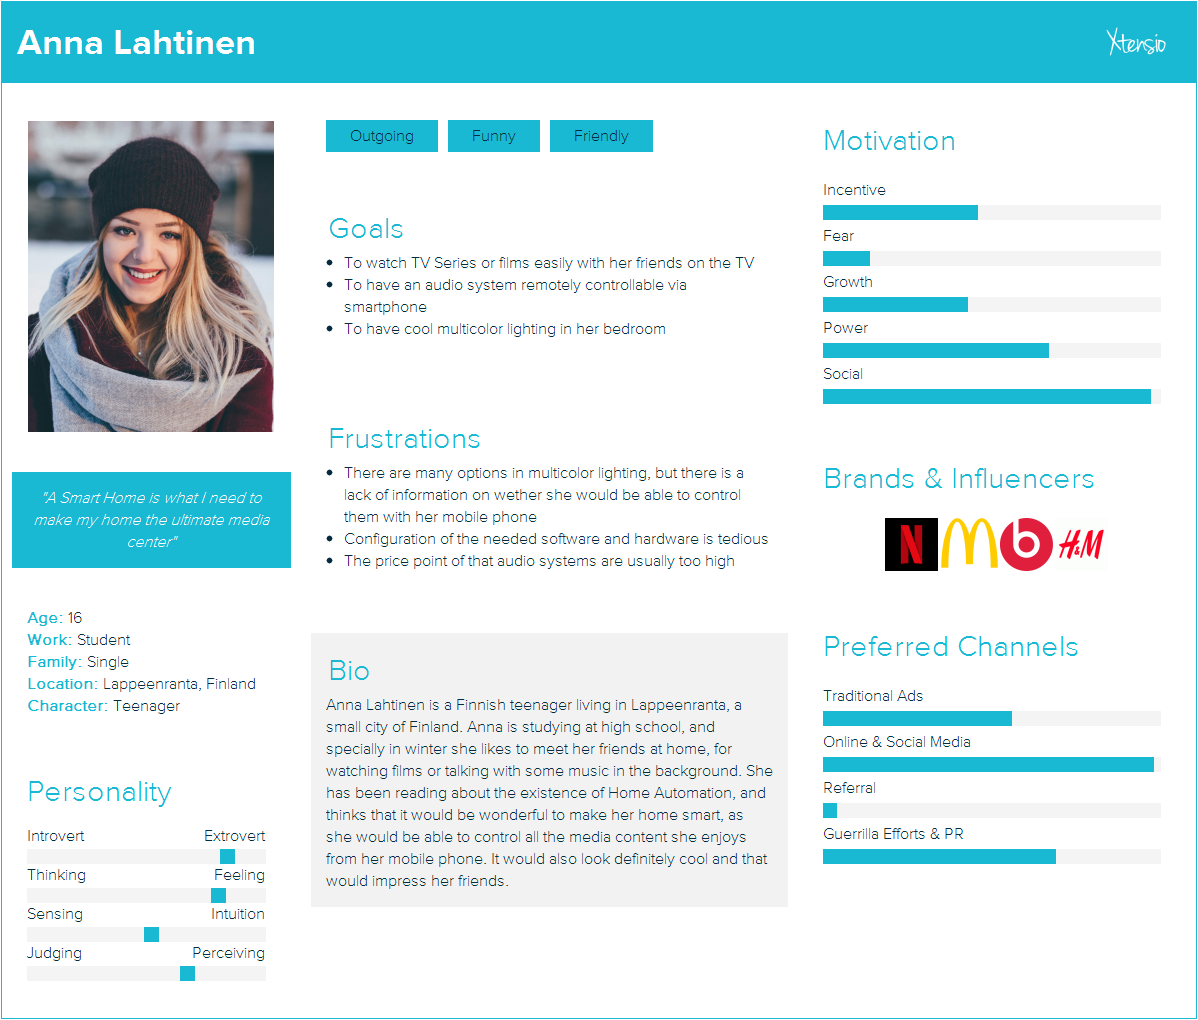
\includegraphics[width=0.65\textwidth]{images/Chapter_06/persona-anna-lahtinen.png}
    \caption{Persona: Anna Lahtinen}
    \label{fig:persona-anna-lahtinen}
\end{sidewaysfigure}

\begin{sidewaysfigure}
    \centering
    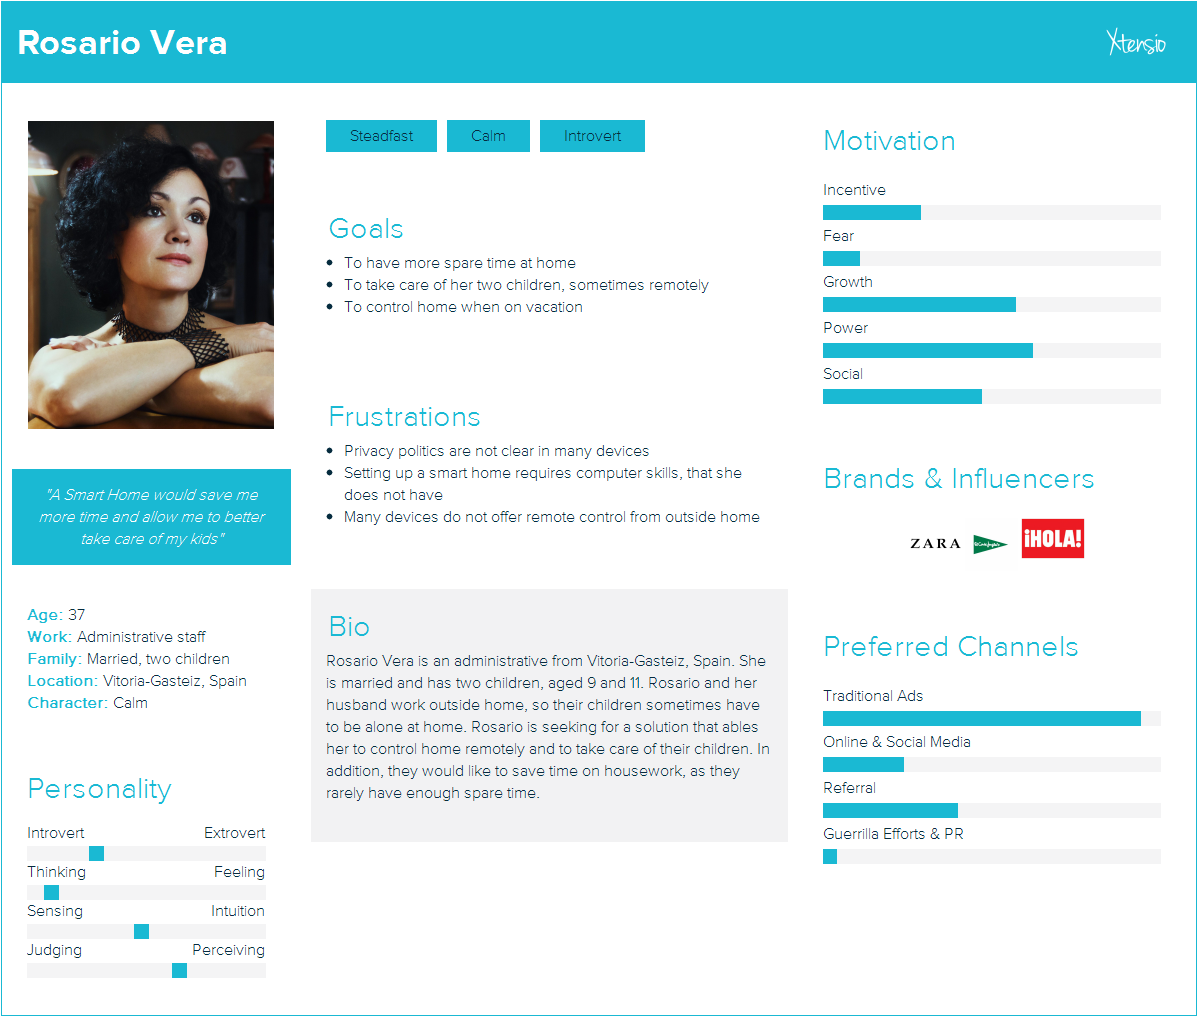
\includegraphics[width=0.65\textwidth]{images/Chapter_06/persona-rosario-vera.png}
    \caption{Persona: Rosario Vera}
    \label{fig:persona-rosario-vera}
\end{sidewaysfigure}

\subsection{Software Requirements Specification}
The Software Requirements Specification (SRS) includes a functional point of view of the project to develop, that is, the capabilities
that the software system will have.

This project focuses on building a home automation controller that can be manageable through new human-computer interaction technologies,
like virtual assistants. The controller will be able to control all modern domotic devices in our home, regardless of their maker and the 
technology they use, as long as it is supported by our system. It will also allow user to add different information, such as the weather 
forecast or the moon phases, from different data providers. It will provide an easy to use user interface and the ability to easily install, 
modify or remove the devices. It will also include natural human-computer interaction through the voice. A more detailed specification 
of the requirements can be found in the subsections below.

\subsubsection{Functional Requirements}
Functional requirements are a description of the facility or feature required. They deal with what the system should do or provide
for users.\cite{sqaFunctionalNonFunctional}

\begin{itemize}
    \item \textbf{FR1}: The system must retrieve automatically the status of the different properties of the devices.
    \item \textbf{FR2}: The system must retrieve automatically data from its different data providers.
    \item \textbf{FR3}: The system must launch openHAB automatically when it is powered on.
    \item \textbf{FR4}: The system must place the home automation runtime in an accessible local server.
    \item \textbf{FR5}: The system must automatically detect new smart devices connected to the local network.
    \item \textbf{FR6}: The system must detect the possible operations with each connected smart device.
    \item \textbf{FR7}: The system must operate with the connected devices according to the detected possible operations.
    \item \textbf{FR8}: The system must tell the user in an understandable manner the current connection status for each
    device.
    \item \textbf{FR9}: The system must provide different user interfaces, so users can choose one between them, according to
    their needs.
    \item \textbf{FR10}: The system must allow the user to change its configuration from a graphical user interface.
    \item \textbf{FR11}: The system must be manually configurable and modifiable using manual configuration files.
    \item \textbf{FR12}: The system must automatically include and configure new devices found in the local network, after the user 
    decides to add them.
    \item \textbf{FR13}: The system must allow the user to configure the name, display icon, IP and all possible aspects of the item 
    directly from the user interface.
    \item \textbf{FR14}: The system must allow the user to group the devices.
    \item \textbf{FR15}: The system must allow the user to add groups of devices to other groups of devices.
    \item \textbf{FR16}: The system must be modular and include a package system. Each package will support a set of devices.
    \item \textbf{FR17}: The package system must be accessible from the graphical user interface.
    \item \textbf{FR18}: The installation of packages must be done automatically after the user clicks on the install button.
    \item \textbf{FR19}: The removal of packages must be done automatically after the user clicks on the remove button.
    \item \textbf{FR20}: The system must maintain an updated and classified list of packages according to an external repository.
    \item \textbf{FR21}: The system must be manageable from external sources.
    \item \textbf{FR22}: The system must allow the access from external devices and from the Internet.
    \item \textbf{FR23}: The system must allow the definition of automation rules.
    \item \textbf{FR24}: The voice assistant must perform the main operations of each device in the system.
    \item \textbf{FR25}: The voice assistant must be able to answer in different languages.
    \item \textbf{FR26}: The voice assistant must do power management tasks in the system, such as powering the system
    off or restarting the system, if asked by the user.
    \item \textbf{FR27}: The voice assistant has to be operable through mechanical methods or by voice.
    \item \textbf{FR28}: The voice assistant functionalities must be editable so users can adapt it to their needs.
    \item \textbf{FR29}: The voice assistant must provide spoken feedback if there has been an error performing the given command.
    \item \textbf{FR30}: The voice assistant must print debug information in the command line if it is required.
\end{itemize}

\subsubsection{Non-Functional Requirements}
Non-functional requirements detail constraints, targets or control mechanisms for the new system. They describe how, how well or
to what standard a function should be provided.\cite{sqaFunctionalNonFunctional}

\begin{itemize}
    \item \textbf{NFR1}: The system, along with the voice assistant, will be installable in the Raspberry Pi.
    \item \textbf{NFR2}: The system and the voice assistant will provide a satisfactory response rate.
    \item \textbf{NFR3}: The user interfaces of the home automation system will be adaptable to the size and resolution of the
    user's screen.
    \item \textbf{NFR4}: The user interfaces will be made according to modern standards, like Material Design.
    \item \textbf{NFR5}: The home automation system will run in a local server, created in the machine which executes it.
    \item \textbf{NFR6}: In order to allow external connections, the home automation system will provide a REST API.
    \item \textbf{NFR7}: The system will provide secure access options.
    \item \textbf{NFR8}: The system must be available the 99\% of the time.
    \item \textbf{NFR9}: The system must be scalable.
    \item \textbf{NFR10}: The system must be recoverable in less than 45 minutes.
    \item \textbf{NFR11}: The cost of the system must me minimal.
    \item \textbf{NFR12}: The system must be interoperable with multiple devices.
    \item \textbf{NFR13}: The voice assistant will recognize English.
    \item \textbf{NFR14}: The voice assistant will be fast in its response. Therefore, its procedure for deciding a response will
    be optimal.
    \item \textbf{NFR15}: The voice assistant will operate with the home automation system via REST, so it can be installed in a
    different computer than the one with the home assistant.
\end{itemize}

\subsection{Use Cases}
The next step after the specification of requirements is to specify the use cases of the system.

Use case diagrams are usually referred to as behavior diagrams used to describe a set of actions (use cases) that some system or
systems (subject) should or can perform in collaboration with one or more external users of the system (actors).\cite{umlUseCaseDiagrams}

\subsubsection{Actor Description}

The Unified Modeling Language (UML)  defines an Actor as an entity that specifies a role played by a user or any other system 
that interacts with the subject.

In this case, we have specified three actors: user, administrator and timer. A description of each one is provided in the tables
\ref{table:actor-1}, \ref{table:actor-2} and \ref{table:actor-3}.

\begin{table}[]
	\centering
	\resizebox{\textwidth}{!}{%
		\begin{tabular}{|l|l|l|l|l|l|}
			\hline
			\textbf{Actor} & \multicolumn{4}{l|}{User} & \cellcolor[HTML]{C0C0C0}AC-1 \\ \hline
			\textbf{Description} & \multicolumn{5}{l|}{Main actor, it can be any person that uses the system} \\ \hline
			\textbf{Characteristics} & \multicolumn{5}{l|}{\begin{tabular}[c]{@{}l@{}}Actor that can perform consultations and modifications over the present\\ domotic devices and their state, as well as over the platform, and the \\ automation rules. The operation with the voice assistant is also allowed\\ to this actor, but not the edition of its parameters.\end{tabular}} \\ \hline
			\textbf{Relationships} & \multicolumn{5}{l|}{} \\ \hline
			\textbf{References} & \multicolumn{5}{l|}{} \\ \hline
			\textbf{Author} & David Vargas Carrillo & \textbf{Date} & 30/08/2018 & \textbf{Version} & 1.0 \\ \hline
		\end{tabular}%
	}
	\caption{Actor 1 definition}
	\label{table:actor-1}
	
	\bigskip
	\centering
	\resizebox{\textwidth}{!}{%
		\begin{tabular}{|l|l|l|l|l|l|}
			\hline
			\textbf{Actor} & \multicolumn{4}{l|}{Administrator} & \cellcolor[HTML]{C0C0C0}AC-2 \\ \hline
			\textbf{Description} & \multicolumn{5}{l|}{\begin{tabular}[c]{@{}l@{}}Actor whose unique purpose is to adapt the voice assistant to the\\ current state of the home automation system\end{tabular}} \\ \hline
			\textbf{Characteristics} & \multicolumn{5}{l|}{\begin{tabular}[c]{@{}l@{}}The administrator is of great importance in this system, as it will be\\ in charge of adapting the voice assistant to the final setup of the\\ home automation system\end{tabular}} \\ \hline
			\textbf{Relationships} & \multicolumn{5}{l|}{User} \\ \hline
			\textbf{References} & \multicolumn{5}{l|}{} \\ \hline
			\textbf{Author} & David Vargas Carrillo & \textbf{Date} & 30/08/2018 & \textbf{Version} & 1.0 \\ \hline
		\end{tabular}%
	}
	\caption{Actor 2 definition}
	\label{table:actor-2}
	
	\bigskip
	\centering
	\resizebox{\textwidth}{!}{%
		\begin{tabular}{|l|l|l|l|l|l|}
			\hline
			\textbf{Actor} & \multicolumn{4}{l|}{Timer} & \cellcolor[HTML]{C0C0C0}AC-3 \\ \hline
			\textbf{Description} & \multicolumn{5}{l|}{This actor performs a task on the system every certain period of time} \\ \hline
			\textbf{Characteristics} & \multicolumn{5}{l|}{\begin{tabular}[c]{@{}l@{}}The timer is an agent on the system that performs repetitive tasks \\ every certain period of time, normally automated tasks related to \\ the current configuration of the system\end{tabular}} \\ \hline
			\textbf{Relationships} & \multicolumn{5}{l|}{User} \\ \hline
			\textbf{References} & \multicolumn{5}{l|}{} \\ \hline
			\textbf{Author} & David Vargas Carrillo & \textbf{Date} & 30/08/2018 & \textbf{Version} & 1.0 \\ \hline
		\end{tabular}%
	}
	\caption{Actor 3 definition}
	\label{table:actor-3}
\end{table}

\subsubsection{Functional Subsystems}
The entire functionality of the system can be encompassed in a set of functional subsystems. From the previously specified use cases, 
we can differentiate four functional subsystems. They are represented in the figure \ref{fig:functional-subsystems}.

\begin{figure}
	\centering
	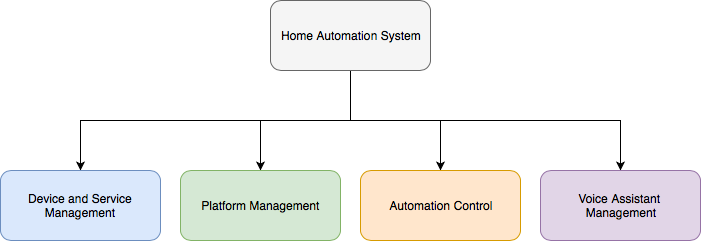
\includegraphics[width=1\textwidth]{images/Chapter_06/functional-subsystems.png}
	\caption{Functional subsystems of the home automation controller}
	\label{fig:functional-subsystems}
\end{figure}

The first functional subsystem is the \textbf{Device and Service Management}, which includes all the functionality related to the 
configured devices and services on the platform, such as their addition, removal and modification. It also includes actions
to update their status on the system and on the physical device. Its use cases are represented in the figure 
\ref{fig:UC-device-and-service-management}.

\begin{figure}
	\centering
	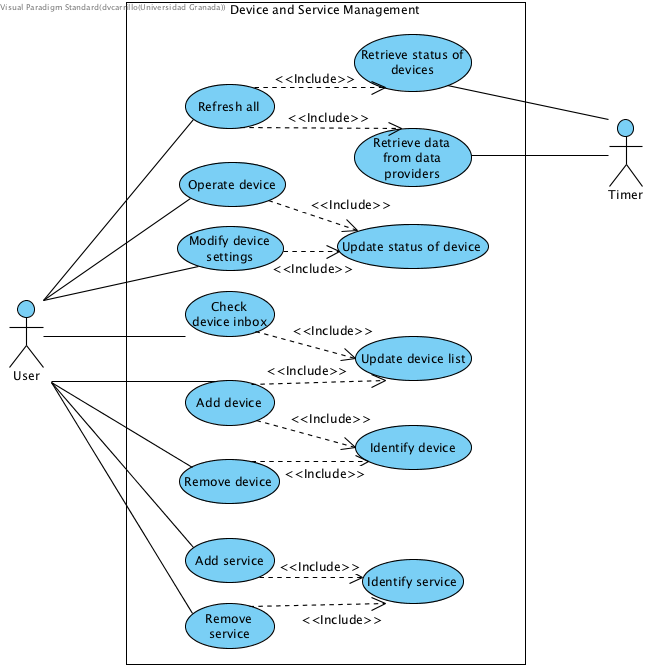
\includegraphics[width=1\textwidth]{images/Chapter_06/UC-device-and-service-management.png}
	\caption{Use cases diagram for the Device and Service Management subsystem}
	\label{fig:UC-device-and-service-management}
\end{figure}

The \textbf{Platform Management} subsystem encompasses the actions aimed to install and uninstall packages to the platform, as well
as all the actions related to change its configuration and the user interface. This subsystem also considers the automatic actions that
are done in order to check for changes in the configuration files that are manually specified. These use cases are depicted in the diagram
in the figure \ref{fig:UC-platform-management}.

\begin{figure}
	\centering
	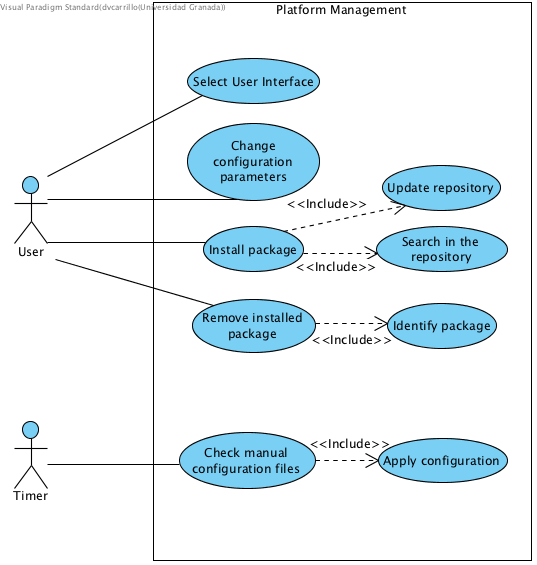
\includegraphics[width=0.8\textwidth]{images/Chapter_06/UC-platform-management.png}
	\caption{Use cases diagram for the Platform Management subsystem}
	\label{fig:UC-platform-management}
\end{figure}

In third place, the \textbf{Automation Control} subsystem comprises the creation, modification and deletion of automation rules that
are set in order to create automatized processes in the system. There are also actions for checking for rules and applying them to 
the devices they are aimed to. The figure \ref{fig:UC-automation-control} includes a diagram of its use cases.

\begin{figure}
	\centering
	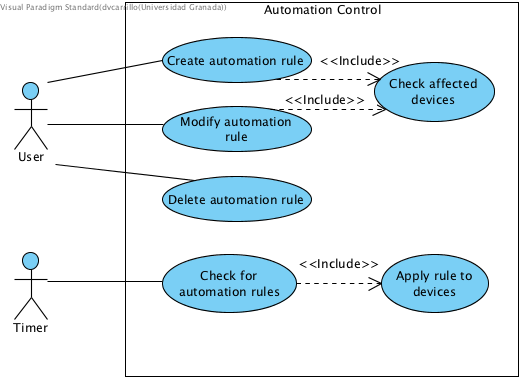
\includegraphics[width=0.8\textwidth]{images/Chapter_06/UC-automation-control.png}
	\caption{Use cases diagram for the Automation Control subsystem}
	\label{fig:UC-automation-control}
\end{figure}

Finally, the \textbf{Voice Assistant} subsystem is in charge of everything related to the voice assistant that interacts with the
home automation system. Very few actions are considered in this subsystem, as its operation is quite simple. It includes actions 
for activating the assistant, sending commands and processing them, and editing their properties. They are represented in the
use cases diagram in figure \ref{fig:UC-voice-assistant-management}.

\begin{figure}
	\centering
	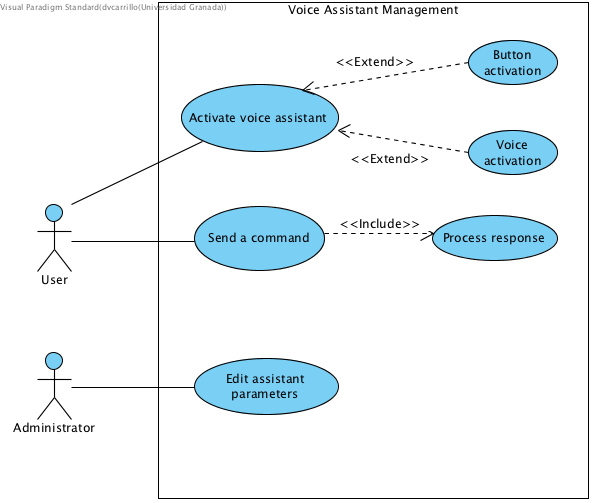
\includegraphics[width=0.8\textwidth]{images/Chapter_06/UC-voice-assistant-management.png}
	\caption{Use cases diagram for the Voice Assistant Management subsystem}
	\label{fig:UC-voice-assistant-management}
\end{figure}

\bigskip
\section{System Design}
Now that we have a clear idea of the product and what users would expect from it, the next step is to design it, that is, to define 
all the characteristics of its elements, how they are going to be connected and how they interact with external systems. This section 
begins defining operating scenarios of this system (how it could be used), then we will specify its architecture from an operating 
scenario, and it ends with the conceptual class diagram of the system.

\subsection{Possible Operating Scenarios}
After exploring what users would expect from a system like this, it is worth thinking about how it should be implemented. We proposed
different options to meet the previous requirements.

\subsubsection{Web Platform}
A well designed web platform is a great idea nowadays. If this platform is hosted in a local server, it means that it can be accessed
from any device connected to the network. With the correct configuration, it could be even reachable from anywhere in the world.
It is easy to implement and maintain, and users with basic web development knowledge would be able to easily modify it. In addition,
the same web platform can be adaptable to any device and resolution, thanks to responsive designs. It would also work if we attach
a tactile screen to the Raspberry Pi.

OpenHAB mounts a web platform in a local server by default, and provides several adaptable user interfaces, so this solution would
not require much effort, and it offers many possibilities.

\subsubsection{Desktop Application}
Another solution, focused on the Raspberry Pi desktop (where we mainly want to implement the system), is developing a desktop
application with an adapted user interface for tactile screens. The advantage of a desktop application is that it usually requires
less resources and it is faster, but it is a specific solution for the Raspberry Pi, so it would only work there. We would need a
different application if we wanted it to run on mobile phones or tablets.

We would need to make it from scratch, as openHAB does not provide any desktop application.

\subsubsection{Mobile Application}
Mobile phones and \textit{tablets} are common devices that are widely used to manage smart homes. Some setups have a tablet located
somewhere in the home, which is only used for managing the domotic devices. An application is faster and more accessible than a web
platform, and users are more used to them, so it would be convenient in some cases.

However, making the system only accessible from a mobile or tablet application would reduce the utility of the Raspberry Pi, and
would at least require two devices (one for the local server and another one for accessing it). Although it is a good complement to the
system, it is not convenient to base it only on a mobile application. However, it is applicable in a hybrid solution.

\subsubsection{Hybrid Solution}
A hybrid solution consists of applying two or more solutions together of those specified above. For example, providing a web platform
and an optional mobile application to easily manage the system from a mobile device.

OpenHAB provides a web platform, as explained above, and a mobile application for iOS and Android than connects to the web platform.

\subsubsection{Comparison}
The table \ref{table:possible-implementations} compares all the possibilities for the implementation of the system.

\begin{table}[]
	\centering
	\resizebox{\textwidth}{!}{%
		\begin{tabular}{|l|c|c|c|c|}
			\hline
			\multicolumn{1}{|c|}{\textbf{Feature}}                                  & \textbf{\begin{tabular}[c]{@{}c@{}}Web\\ platform\end{tabular}} & \textbf{\begin{tabular}[c]{@{}c@{}}Desktop \\ application\end{tabular}} & \textbf{\begin{tabular}[c]{@{}c@{}}Mobile\\ application\end{tabular}} & \textbf{\begin{tabular}[c]{@{}c@{}}Hybrid\\ Solution\end{tabular}} \\ \hline
			\begin{tabular}[c]{@{}l@{}}Support for \\ multiple devices\end{tabular} & Yes                                                             & Only PCs                                                                & \begin{tabular}[c]{@{}c@{}}Only mobile\\ phones/tablets\end{tabular}  & Yes                                                                \\ \hline
			\begin{tabular}[c]{@{}l@{}}Allows access\\ from Internet\end{tabular}   & Yes                                                             & No                                                                      & No                                                                    & Yes                                                                \\ \hline
			\begin{tabular}[c]{@{}l@{}}Control from\\ Raspberry Pi\end{tabular}     & Yes                                                             & Yes                                                                     & No                                                                    & Yes                                                                \\ \hline
			\begin{tabular}[c]{@{}l@{}}Easy \\ implementation\end{tabular}          & Yes                                                             & No                                                                      & No                                                                    & Yes                                                                \\ \hline
			\begin{tabular}[c]{@{}l@{}}Maximum\\ performance\end{tabular}           & No                                                              & Yes                                                                     & Yes                                                                   & Partially                                                          \\ \hline
		\end{tabular}%
	}
	\caption{Comparison between possible implementations}
	\label{table:possible-implementations}
\end{table}

As we can see, the hybrid solution, which is a web platform and mobile application, meets all the features in the best way, and
offers easy and fast implementation. This solution will be complemented with a virtual assistant.

\subsection{Architecture}
The architecture of the hybrid solution, considering it as a conjunction of the web platform and the mobile application, plus the voice
assistant, is described in the figure \ref{fig:system-architecture}. 

\begin{figure}
	\centering
	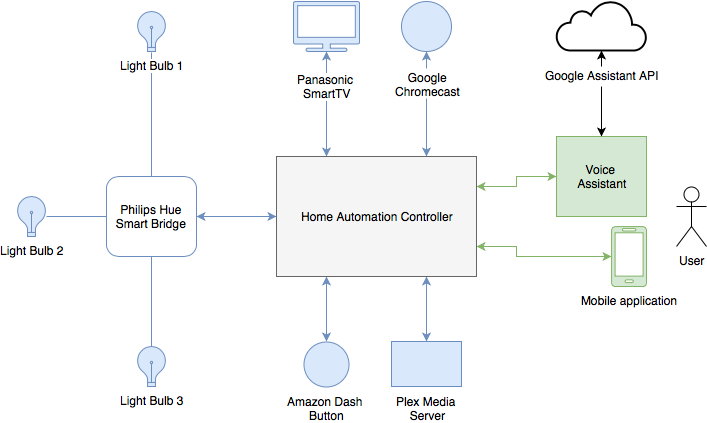
\includegraphics[width=1\textwidth]{images/Chapter_06/system-architecture.png}
	\caption{Architecture of the home automation system}
	\label{fig:system-architecture}
\end{figure}

\bigskip
\section{Implementation}
In this section, we will explain the process that we have followed to implement the home automation controller, along with the voice
assistant.

\begin{figure}
    \centering
    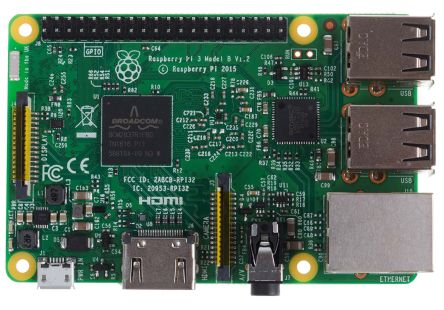
\includegraphics[width=0.8\textwidth]{images/Chapter_06/raspberry-pi-3b.jpg}
    \caption{Raspberry Pi 3 Model B}
    \label{fig:raspberry-pi-3b}
\end{figure}

As mentioned before, the main objective is to install the system in a Raspberry Pi, which is an affordable and small computer,
with enough power and connectivity options to install a home automation system on it, and even a voice assistant. The possibilities
of this device are endless: it can work with or without display, and has a special connector to which the user can connect screens,
microphones, speakers and many other accessories. It also has USB ports on its high-end models, and accepts all the USB
accessories that a normal computer would accept.\cite{raspberryPiDocs}

The first approach to this system was to install Raspbian, a Linux distribution provided by openHAB, over a Raspberry Pi 3 Model B
(figure \ref{fig:raspberry-pi-3b}). Raspbian has openHAB preinstalled and configured, so it is ready to use. The first idea was to
have a computer with openHAB and then a voice assistant in other machine. We installed the distribution on this mini PC, but after
reviewing the possible voice assistants, we found that it was not the best way to implement it.

We found the Google AIY Voice Kit, which is a kit provided by Google to makers that want to play around with voice recognition.
They provide a package with some accessories for the Raspberry Pi and a cardboard box that is meant to contain the board and the
accessories. Then, we reconsidered the architecture. It would be also possible to install openHAB in the same machine as the virtual
assistant. This way, we would need just one machine for all. It would be a voice assistant, but with a local server, accessible from
all the devices connected to the local network. It would be possible to attach a screen to it as well, so the user can manage the
smart home graphically from the same device.

We thought this would be the best solution, and it would still meet all the requirements specified previously. So, we began working
on it.

\subsection{Introduction to Google AIY Voice Kit}
The AIY Voice Kit is a do-it-yourself project created by Google that demonstrates how easy and inexpensive can be to create a natural
voice recognizer that works with Google Assistant, at a price of only EUR 30 in Europe. The project, aimed for makers, also lets the
user add their own questions, which is the most powerful part for our purpose.

The idea is to adapt the device in order to fetch the voice commands that the microphone captures and manage them in openHAB,
making the system act following user’s instructions.

\subsubsection{Capabilities}
The main advantage of the Google AIY Voice Kit, and the reason why we have chosen it for this project, is that we can access the
Google Cloud Voice API and create our own voice interfaces. Everything is coded in Python, and we can create voice commands to
control it.

This, along with the more than reasonable quality of its stereo microphone and speaker, make it a very useful device that could
perfectly fit in a smart home, despite its looks.

The device is capable of recognizing the “OK Google” command, as well triggering the assistant when the big red button is pressed,
and, by default, it is capable of doing almost everything that the Google Assistant on smartphones can do, including integration
with the apps in the user’s smartphone and reading the news, among other things.

\subsubsection{The Main Challenge}
The challenge is to explore how Google AIY Voice Kit and openHAB 2, both installed on the same system, can work together and,
if it is possible, connect them so a standard user can control its smart home using voice commands and universal, open source solutions.

\subsection{Building the Google AIY Voice Kit}
For making the voice recognizer, we primarily used:

\begin{itemize}
    \item Cardboard for the body of the device.
    \item A speaker.
    \item A Voice HAT microphone board and an accessory board.
    \item A big button with a light inside to trigger the voice recognition.
    \item A Raspberry Pi Model 3 B.
    \item An 8GB microSD card.
    \item Cables to connect everything.
\end{itemize}

\begin{figure}
    \centering
    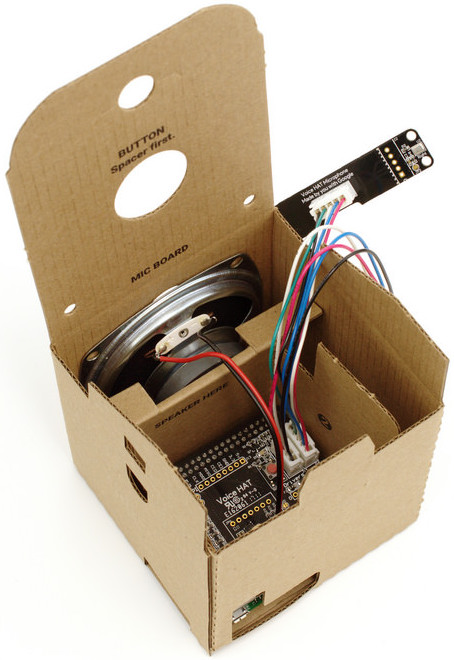
\includegraphics[width=0.5\textwidth]{images/Chapter_06/aiy-voice-kit.jpeg}
    \caption{The AIY Voice Kit}
    \label{fig:aiy-voice-kit}
\end{figure}

First of all, we had to put all the items together and assemble the cardboard body. The Voice HAT accessory board is connected to the
Raspberry Pi through its GPIO connector, which is adapted to connect the rest of devices: the speaker, the microphone board and the
button. Once everything was correctly connected, we had to assemble the cardboard body, which was composed by two
pieces.\cite{aiyProjectsVoice}

The next step was to write the Voice Kit SD image\cite{voiceKitSdImage} to the microSD card. The \textit{Etcher.io} macOS application
was used for this purpose.

The system includes everything that the Raspberry Pi needs to use the connected devices, so we only needed to check that they worked
fine and were correctly connected. The system also includes two demos with Google Assistant: one that triggers the assistant by saying
“OK Google!”, and another that needs the button to be pressed to trigger it.

To make any demo or a new app that uses Google Assistant work, it is necessary to register a new project on Google Cloud Platform
(GCP) first. A project of this kind has to include the Google Assistant API, which can be enabled via GCP, as well as an OAuth 2.0
client. Finally, at the moment of running the application, it seeks a JSON file that contains all this information. By default, it
must be placed in the home folder and it must be called assistant.json.

Google Assistant gathers all the user’s information from their Google account, so they must have enabled the web and app activity,
the device information and the voice and audio activity from their Activity Controls panel in their Google account settings.

\subsection{Setting up openHAB 2}
In this case, the goal is to install openHAB in the Linux distribution that the AIY Kit provides, which is a fork of Raspbian
(that is a fork of Debian made for the Raspberry Pi), with the suitable drivers in order to support all the accessories from the kit.
Luckily, openHAB provide in their documentation pages\cite{openHABDocs} enough instructions to make this process easier.

In this process, we used a keyboard and a mouse for interacting with the operating system, but it can also be done remotely via
SSH connection.

As a prerequisite, Java 8 must be installed on the system. Users may prefer Zulu, the main Java \textit{alternative}, a fully
certified build of OpenJDK.\cite{zuluWebsite}

OpenHAB 2 can be installed though a package repository or manually from file, but it is recommended to install through a package
repository, using \textit{apt}, \textit{apt-get}, \textit{yum} or \textit{dnf}. As this operating system is based on Debian, we
used \textit{apt-get}.

First of all, we have to add the openHAB 2 Bintray repository key to the package manager and allow \textit{apt} to use the HTTPS
Protocol.

\begin{lstlisting}[style=Consola]
wget -qO - 'https://bintray.com/user/downloadSubjectPublicKey?username=openhab' | sudo apt-key add -
sudo apt-get install apt-transport-https
\end{lstlisting}

OpenHAB offers Stable (Official), Beta and Snapshot builds to choose from. The stable builds contain the latest official release
with tested features, so it is the \textit{safest} to use. We will install this one. Then, we need to add the openHAB 2 Stable Repository
to system's apt sources list:

\begin{lstlisting}[style=Consola]
echo 'deb https://dl.bintray.com/openhab/apt-repo2 stable main' | sudo tee /etc/apt/sources.list.d/openhab2.list
\end{lstlisting}

Next, we have to resynchronize the package index:

\begin{lstlisting}[style=Consola]
sudo apt-get update
\end{lstlisting}

And now we can install openHAB:

\begin{lstlisting}[style=Consola]
sudo apt-get install openhab2
\end{lstlisting}

Optionally, it is possible to install the add-ons package (\textit{openhab2-addons}), but it is meant to be installed if the machine
is going to be disconnected from the Internet, as openHAB downloads them on request by default. In this case, we assume that the
system is always going to be connected to Internet.

At this point, we can start openHAB and register it to be automatically executed at system startup. To this end, the documentation
provides the following commands for systems based on \textit{systemd}, such as Raspbian.

\begin{lstlisting}[style=Consola]
sudo systemctl start openhab2.service
sudo systemctl status openhab2.service

sudo systemctl daemon-reload
sudo systemctl enable openhab2.service
\end{lstlisting}

After some minutes, openHAB is ready on the local server, in the port 8080 (accessible in \textit{http://localhost:8080}). Then,
the following commands are used to control the service.

\begin{figure}
    \centering
    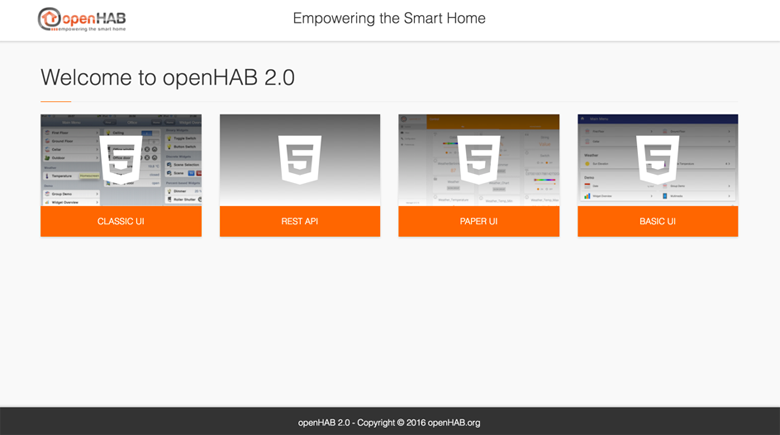
\includegraphics[width=1\textwidth]{images/Chapter_06/openhab-startup.png}
    \caption{OpenHAB 2 startup screen}
    \label{fig:openhab-startup}
\end{figure}

\begin{lstlisting}[style=Consola]
# Current service status
sudo /etc/init.d/openhab2 status

# (Re-)Start openHAB (background service)
sudo /etc/init.d/openhab2 restart

# Stop the openHAB background service
sudo /etc/init.d/openhab2 stop

# Make openHAB automatically start after booting the Linux host
sudo update-rc.d openhab2 defaults
\end{lstlisting}

OpenHAB installs also a utility in the command line interface, named \textit{openhab-cli}, that provides access to the openHAB-specific
commands.

\begin{lstlisting}[style=Consola]
Usage:  openhab-cli command [options]

Possible commands:
  start [--debug]     -- Starts openHAB in the terminal.
  stop                -- Stops any running instance of openHAB.
  status              -- Checks to see if openHAB is running.
  console             -- Opens the openHAB console.
  backup [filename]   -- Stores the current configuration of openHAB.
  restore filename    -- Restores the openHAB configuration from a backup.
  showlogs            -- Displays the log messages of openHAB.
  info                -- Displays distribution information.
\end{lstlisting}

Lastly, to stay up to date to new releases, they recommend to execute the following commands periodically. Note that this also applies
to the rest of the packages installed in the Linux system.

\begin{lstlisting}[style=Consola]
sudo apt-get update
sudo apt-get upgrade
\end{lstlisting}

\subsection{Adding Philips Hue Devices}
Now that we have openHAB 2 up and running in the Raspberry Pi integrated in the AIY Kit, it is desirable to add a device to the home
automation system. We have a Philips Hue lightning system available, so in this section we will explain the process that we have
followed to add it and configure it in our openHAB 2 instance.

\subsubsection{The Hue System}
Our Philips Hue system is composed by the \textit{white and color ambiance starter kit}\cite{philipsHueMeethue} (which consists
in three Hue white and color lights and a Hue hub) as well as a Hue motion sensor:

\begin{itemize}
    \item \textbf{The Hue Hub} acts as a bridge between the user interface (the smartphone application or the OpenHab instance) and
    the connected devices. It is configured and controlled via the Hue app and supports up to 50 lights at the same time. It communicates
    via Zigbee with the Hue devices.
    \item \textbf{The Hue Motion Sensor} can be configured to turn on and off the lights when it detects movement and under some
    defined conditions. By default, it is configured from the Hue app.
    \item \textbf{The Hue White and Color Lights} are customizable RGB lights. By default, they are configurable from the Hue app,
    which offers many ways of changing the light emission.
\end{itemize}

\subsubsection{Installation and Configuration Process on PaperUI}
Philips, as many other companies, is restrictive regarding their home automation devices, and every communication between the Hue
devices and the controller (openHAB in this case) needs to pass through the Hue Hub. The Hub communicates via WiFi with the controller
and via Zigbee with the Hue devices. The software it uses is privative, but luckily openHAB 2 implements protocols that make possible
the communication between the controller and the Hub. This makes the Hub, though, a frustrating addition to our home automation system.

The Hue system needs to be configured from the Philips Hue mobile application in the first place. This process will link the Hub with the
desired Hue devices, so the next time that the user connects to the Hub, it will not be necessary to configure them again, even if
the connection is done from openHAB. The application allows to manage rooms and sort the devices, as well as setting automated commands
(for instance, turning the light on when the motion sensor detects any movement). OpenHAB is unable to perform such complex operations
by default, providing only a few channels for the light bulb.

Once the Hub is on, connected and linked with the Hue devices, we can proceed to configure it on openHAB. In this case, we explain
the process to follow in order to add the light bulb controls, but it might work for other Hue devices in a future. If openHAB is
used on a system connected to the same network as the Hub, the Hub will automatically appear in the \textit{Inbox} section. We have
to make sure before that its related binding. Adding the Hub in the Inbox section means that it will be listed as a Thing. OpenHAB
takes care automatically of the Thing (figure \ref{fig:philips-hue-hub-thing}) and Items configuration. After adding them, the host
device and the Hub will be able to communicate between them. However, the user needs to press the pairing button on the Hub in
order to activate the communication.

\begin{figure}
    \centering
    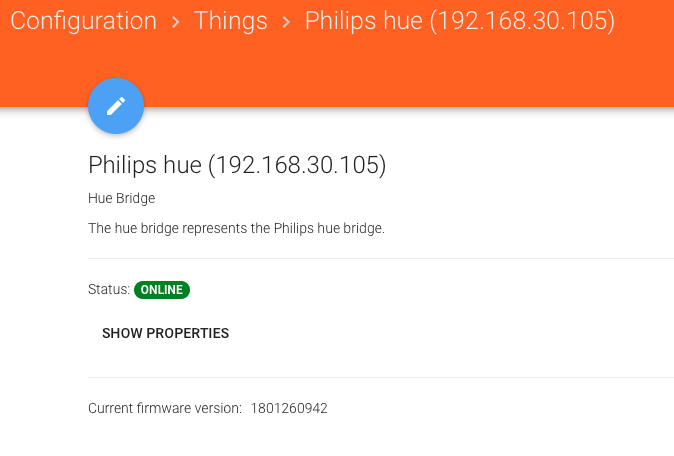
\includegraphics[width=0.9\textwidth]{images/Chapter_06/philips-hue-hub-thing.png}
    \caption{Philips Hue Hub Thing}
    \label{fig:philips-hue-hub-thing}
\end{figure}

After that, the Hub will act as a bridge and openHAB will be able to display all the compatible devices connected to the Hub. In
this case, the Hue color lamp appears in the Inbox. The process for adding it is the same as with the Hub. Nevertheless, this time
the light controls will be added automatically to the Control panel according to the linked channels on the thing. OpenHAB supports
two channels that are directly related to the bulb functionality: \textit{color} (which is divided in tone, brightness and saturation)
and \textit{white temperature}. The first one will set the light in a color with the desired properties, and the second will set a
white color from a range of whites (from cold to warm white). Additionally, OpenHAB provides two more channels: \textit{alert},
to use the bulb as an alert light under certain circumstances, and \textit{color loop}, which will make the light color iterate in
the whole color spectrum. The figure \ref{fig:hue-color-bulb-channels} shows the PaperUI interface showing these channels.

\begin{figure}
    \centering
    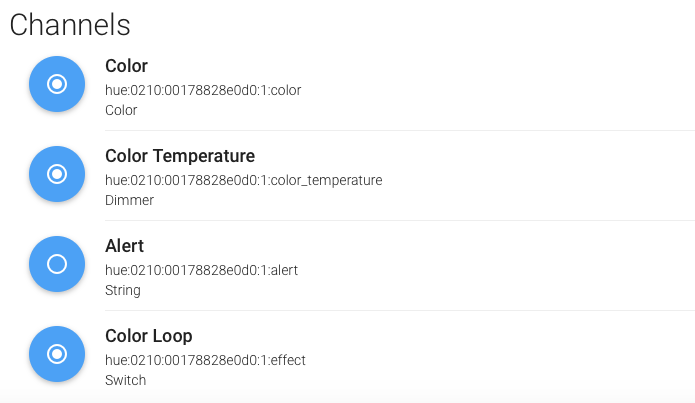
\includegraphics[width=0.9\textwidth]{images/Chapter_06/hue-color-bulb-channels.png}
    \caption{Available channels in the Hue color bulb}
    \label{fig:hue-color-bulb-channels}
\end{figure}

\begin{figure}
    \centering
    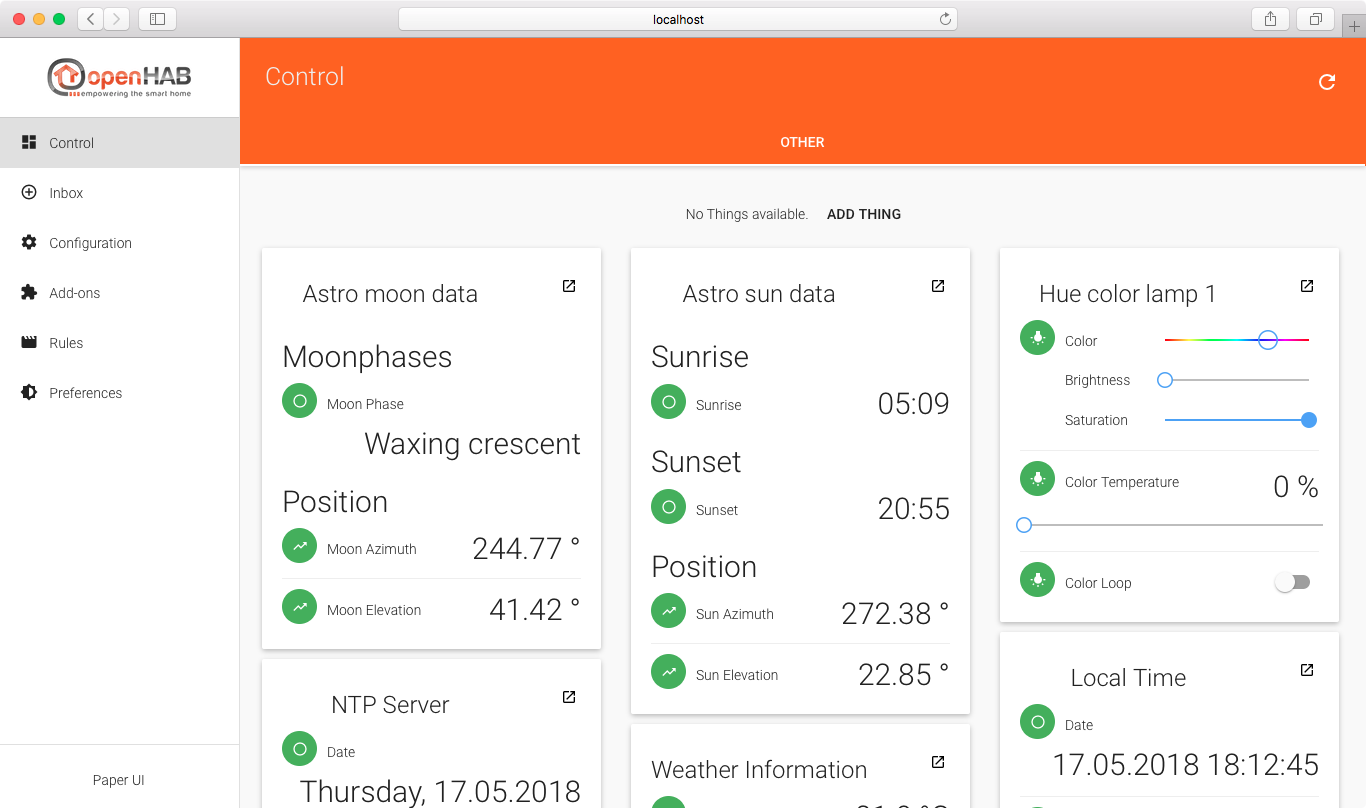
\includegraphics[width=1\textwidth]{images/Chapter_06/openhab-control-hue.png}
    \caption{OpenHAB 2 Control Panel with the Hue color bulb controls}
    \label{fig:openhab-control-hue}
\end{figure}

\subsubsection{Internal Functionality}
OpenHAB is able to communicate with the Hue Hub and Hue devices thanks to the Philips Hue binding (represented as a set of packages
in Java, as shown in the figure \ref{fig:hue-binding-structure}), integrated in the Eclipse SmartHome Extensions repository.

\begin{figure}
    \centering
    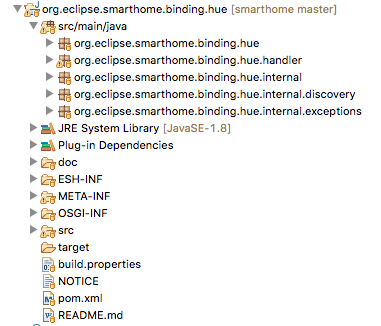
\includegraphics[width=0.6\textwidth]{images/Chapter_06/hue-binding-structure.png}
    \caption{Philips Hue binding internal structure}
    \label{fig:hue-binding-structure}
\end{figure}

As we can see, there are packages for handling the lights and Hub (which is named \textit{bridge}), and for managing the internal
functionality of the binding and openHAB. That is, discovering the devices and showing them in the Inbox and managing exceptions.
Examples of exceptions can be having the device off or sending the device a wrong command.

Looking more closely at the device handlers, we can see that the bridge handler implements a \textit{Runnable} object with a
\textit{run} method, which gets the Hub configuration. The function gets the IDs of all the lights connected to the Hub and iterates
over them. If a light is not listed in a list of light states caught from openHAB, it is added as a new light. If it is listed, then
it checks for changes in the status of the light, comparing the actual state with the last one saved. If the states are different,
notifies the Light listeners. There is a \textit{LightStatusListener} interface that is called on each change, it will modify the
Light and Hue objects.

\subsection{Specifying Items Manually}
In previous chapters, we introduced the concept of Item in openHAB 2. Items represent functionalities that can be used by the
applications, mainly user interfaces or automation logic.

OpenHAB is able to configure many Things and Items automatically in the PaperUI. But in many cases we may need to specify Items
manually. For example, for creating custom views(sitemaps), as we will see below. Therefore, it is important to know how to specify
Items manually.

First of all, we need to create an Items file. Both the items and the sitemap files are located in the \$OPENHAB\_CONF directory,
which is different on different operating systems. In our case, they are located in:

\begin{lstlisting}[style=Consola]
/usr/share/openhab2/conf/items       <-- *.items files
/usr/share/openhab2/conf/sitemaps    <-- *.sitemap files
\end{lstlisting}

After a fresh installation these directories are empty (except for the \textit{readme} files), so we have to create a file there.
It will be called \textit{default.items} in this case.

OpenHAB has its own syntax for defining Items and Sitemaps, but it is very easy to use. The basic syntax for defining an item is:

\begin{lstlisting}[style=Consola]
ItemType ItemName "ItemDescription" <ItemIcon> {ItemToThingChannelLink}
\end{lstlisting}

The code we have used for defining the item linked to the color channel and the item linked to the white tone channel of a Philips
Hue color bulb is the following:

\begin{lstlisting}[style=Consola]
Color HueColor1 "Hue Light Bulb 1 Color" <lightbulb> {channel="hue:0210:00178828e0d0:1:color"}

Dimmer HueDimmer1 "Hue Light Bulb 1 Temperature" <lightbulb> {channel="hue:0210:00178828e0d0:1:color_temperature"}
\end{lstlisting}

Now, these Items are registered in the system, but before we can see them, we have to define a sitemap and include them there.

\subsection{Creating a Sitemap}
PaperUI, the newest addition in openHAB 2, is meant to make easier the device management, configuration and discovery. Many of
these processes are carried out seamlessly, without user intervention. But this user interface lacks some functionalities, such as
custom ordering of Things. \textit{Sitemaps} are custom views that can be displayed in another user interface, the Basic UI, which
is also automatically installed at the beginning.\cite{openHABDocs} Sitemaps take defined Items and display them as the user specifies
in the UI.

The user is able to define as many sitemaps as desired, and they can be selected from openHAB 2 home screen, in the Basic UI. Sitemaps
are text files with the \textit{.sitemap} extension, and they are defined in the folder specified in the previous section, inside the
openHAB installation directory.

The basic syntax that a sitemap follows is:

\begin{lstlisting}[style=Consola]
sitemap <sitemapname> label="<title of the main screen>"
{
    [all sitemap elements]
}
\end{lstlisting}

Sitemaps are composed by arranging various user interface elements. A set of different element types supports a user-friendly and
clear presentation. One line of Sitemap element definition produces one corresponding UI element. As shown in the example on the
figure \ref{fig:hue-bulb-sitemap}, each element generates a descriptive text next to an icon on the left side and a status and/or
interaction elements on the right.

A certain set of parameters can be configured to customize the presentation of an element. In the shown example \textit{item} and
\textit{icon} are parameters. Almost all parameters are optional, some are however needed to result in a meaningful user interface.

By encapsulating elements with curly brackets, multiple elements can be nested inside or behind others. The Frame element type is
often used in combination with element blocks. Frames are used to visually distinguish multiple elements of the same topic on one
interface page. When using code blocks behind other element types such as \textit{Text}, \textit{Group} or \textit{Switch}, these UI
elements will, in addition to their normal function, be links to a new view, presenting the nested elements. In the example in
\ref{fig:hue-bulb-sitemap}, we created a single Frame that represented all the functionalities of the Hue Color Light.

The \textit{sitemap} element is mandatory in a Sitemap definition. This element shall be the first line in the sitemap file, and the
following code block comprises the entire Sitemap definition.\cite{openHABDocs}

\begin{figure}
    \centering
    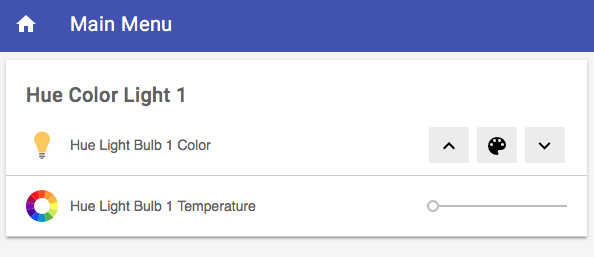
\includegraphics[width=0.9\textwidth]{images/Chapter_06/hue-bulb-sitemap.png}
    \caption{Basic UI displaying a Hue Color Light Item}
    \label{fig:hue-bulb-sitemap}
\end{figure}

From the previous example, we built a sitemap that could display the Hue color light Item previously configured in the Basic UI.
The figure \ref{fig:hue-bulb-sitemap} shows the result of introducing the following code in a file that we called \textit{default.sitemap}.

\begin{lstlisting}[style=Consola]
sitemap demo label="Main Menu"
{
    Frame label="Hue Color Light 1" {
        Colorpicker item=HueColor1 icon="slider"
        Slider item=HueDimmer1 icon="colorwheel"
    }
}
\end{lstlisting}

A frame is containing the main functionality of the Hue color light bulb, and that can be done for every new component installed at home.

OpenHAB 2 allows us to group our items so we can sort them by room or type. That can be made through the Group Item type.

\subsubsection{Elements on a Sitemap}
The element types specified in the table \ref{table:openhab-sitemaps-types} may be used in a Sitemap definition file.

\begin{table}[]
    \centering
    \resizebox{\textwidth}{!}{%
        \begin{tabular}{|l|l|}
            \hline
            \multicolumn{1}{|c|}{\textbf{Type}} & \multicolumn{1}{c|}{\textbf{Description}} \\ \hline
            Chart & Adds a time-series chart object for persisted data \\ \hline
            Colorpicker & Allows the user to choose a color from a color wheel \\ \hline
            Default & \begin{tabular}[c]{@{}l@{}}Renders an Item in the default UI representation specified \\ by the type of the given Item\end{tabular} \\ \hline
            Frame & \begin{tabular}[c]{@{}l@{}}Establishes an area containing various other Sitemap \\ elements\end{tabular} \\ \hline
            Group & \begin{tabular}[c]{@{}l@{}}Concentrates all elements of a given group in a nested \\ block\end{tabular} \\ \hline
            Image & Renders an image given by an URL \\ \hline
            Mapview & Displays an OSM map based on a given Location Item \\ \hline
            Selection & \begin{tabular}[c]{@{}l@{}}Provides a dropdown or modal popup presenting values\\ to choose from for an Item\end{tabular} \\ \hline
            Setpoint & \begin{tabular}[c]{@{}l@{}}Renders a value between an increase and a decrease \\ buttons\end{tabular} \\ \hline
            Slider & Presents a value in a progress-bar-like slider \\ \hline
            Switch & Renders an Item as an ON/OFF or multi-button switch \\ \hline
            Text & Renders an Item as text \\ \hline
            Video & Displays a video stream, given a direct URL \\ \hline
            Webview & Displays the content of a webpage \\ \hline
        \end{tabular}%
    }
    \caption{Types of elements for a Sitemap in openHAB 2}
    \label{table:openhab-sitemaps-types}
\end{table}

Data presented by Sitemap elements will almost always originate from a referenced Item. Each Item is of a certain Item type, for
example \textit{Switch}, \textit{Number} or \textit{String}.

While not all combinations are meaningful, Items of one \textit{datatype} may be linked to different Sitemap element types. This
provides the flexibility to present Items in the way desired in the home automation user interface.

\bigskip
At this point, we have openHAB installed in the Raspberry Pi inside the AIY Voice Kit. OpenHAB is communicating with the Hue Hub and
the Hue Color Light, and its state can be changed by accessing to the server that openHAB has created in the local network. This means
that, if we type on the browser of the mobile phone the IP address of openHAB and its port (8080), we will be able to control the light
from the phone as well. The state of the bulb can be changed from PaperUI (with the view that it has generated automatically) and from
Basic UI, with the view and Items that we have specified in these previous steps.

Now the challenge is to build an assistant that can communicate with openHAB, and that is able to change the state of the configured
Items.

\subsection{Voice Assistants and Speech-To-Text Services}
The Google AIY Voice Kit, the device we are building the system on, already provides some files to access the Google Assistant. This
means that, by default, it can work just like any Google Home device (we explored these devices in previous chapters), so it can
provide general information and knowledge, play songs and tell the weather forecast, among other things. The files that the AIY Voice
Kit provide are accessible and modifiable, so we could write an assistant that would work on top of the Google Assistant, with special
commands.

\subsubsection{Introduction}
We could divide a simple voice assistant, like the one we are building on top of the Google Assistant for managing openHAB and the
Raspberry Pi, in three different parts:
\begin{enumerate}
    \item Speech-To-Text (STT) conversion.
    \item Command processing.
    \item Text-To-Speech (TTS) conversion.
\end{enumerate}

The flow after each command from the user follows the order above. On the next few lines, we are going to explain a little further
each one of these points.

\subsubsection{Speech-To-Text}
The Speech-To-Text or STT comes from the Speech Recognition, a sub-field of computational linguistics and IA. It is a computer
technique that enables the recognition and transcription of spoken language into text by analyzing the captured audio.

It is the first step on the machine after capturing the voice, and it requires the execution of complex algorithms. This is why many
companies, like Google, offer “cloud speech recognition”, where the audio is entirely processed in the cloud, taking advantage of
very powerful computers. Thanks to this, its precision is much higher than other local solutions.

\subsubsection{Command Processing}
Once the system has the transcription of the spoken command, it must relate it with an action. It can be the execution of a function,
or just a spoken response, or both. The complexity of this part can vary significantly, depending on the range of actions we would
like the assistant to perform, or on how specific we want to be when recognizing the language.

There are grammar specifications and even XML dialects for this purpose, like AIML. For the custom assistant we have built, we also
propose a model for processing the speech, as we will mention in further sections.

\subsubsection{Text-To-Speech}
Text-To-Speech or TTS is the inverse process of STT, that is, the artificial production of human speech given a text through a
number of processes that produce a pronounceable version of the text and a digital sound, thanks to signal treatment techniques.

It is often the final step in the interaction with an assistant, when the assistant gives a response to a command given by the user.

\subsubsection{STT and TTS in the Custom Assistant}
The part where we have researched the most, which is also the one that offers more possibilities to this kind of assistant, is the
speech recognition. We have found plenty of services that offer this technology, locally and in the cloud. Many of them work on
Raspberry Pi, the heart of the Google AIY Kit.

Google integrates in this kit the integration with two STT services: the Google Assistant Library and the Google Cloud
Speech-To-Text API\cite{googleCloudSttWebsite}. Both of them make the transcription in the cloud, freeing the Raspberry Pi from
using much processing power in it. Both of them are truly accurate and rarely produce a wrong result, as it is expected from Google.
Using this implementation of the Google Assistant Library is free, but it only works in English at this moment, so it is only
possible to make the assistant in this language with this service. On the other hand, the Google Cloud Speech API is capable of
recognizing more than 120 languages with its variants, even with long audio files. It can also provide content filters and automatic
punctuation. But this solution is not totally free, it comes with a price of \$0.006 USD per 15 seconds of audio after 60 minutes,
each month.\cite{craftworkzBlog}\cite{globalmeBlog}

Outside of Google, there are many other services that could also work with our assistant, from local solutions like
CMUSphinx\cite{cmusphinxWiki} to cloud services provided by other companies. Local solutions offer offline recognition, in
exchange for taking up large storage space and being slower and a lot more inaccurate than the cloud ones. Furthermore,
cloud services are constantly updated and offer state-of-the-art voice recognition. They are usually very fast and, as they work
in the cloud, do not need space on the user's drive. Usually, the providers of these services are major technology companies
such as Microsoft and IBM\cite{ibmWatsonSttWebsite}, which provide the API for a periodic fee.

To find out which service best fits in our custom assistant, we compare the most interesting ones we have found in the table
\ref{table:comparison-stt-services}.

\begin{table}[]
    \centering
    \resizebox{\textwidth}{!}{%
        \begin{tabular}{|l|l|l|l|l|}
            \hline
            \textbf{Name} & Assistant Library & Cloud TTS\cite{googleCloudSttWebsite} & Pocketsphinx\cite{cmusphinxWiki} & Watson STT\cite{ibmWatsonSttWebsite}\cite{ibmDeveloperWorksRecipes} \\ \hline
            \textbf{Maker} & Google & Google & CMUSphinx & IBM \\ \hline
            \textbf{Location} & Cloud & Cloud & Local & Cloud \\ \hline
            \textbf{\begin{tabular}[c]{@{}l@{}}Voice HAT\\ support\end{tabular}} & Yes & Yes & No & No \\ \hline
            \textbf{\begin{tabular}[c]{@{}l@{}}Required \\ space\end{tabular}} & Insignificant & Insignificant & \begin{tabular}[c]{@{}l@{}}40 MB +\\ language models\end{tabular} & Insignificant \\ \hline
            \textbf{\begin{tabular}[c]{@{}l@{}}Recognition\\ quality\end{tabular}} & Excellent & Excellent & Good & Excellent \\ \hline
            \textbf{Languages} & English & 120 supported & 13 supported\footnotemark & 13 supported \\ \hline
            \textbf{Prince} & \begin{tabular}[c]{@{}l@{}}Free (comes with\\ the AIY Kit)\end{tabular} & \begin{tabular}[c]{@{}l@{}}\$0.006 USD/15 \\ seconds after 60 \\ minutes/mo.\end{tabular} & Free & \begin{tabular}[c]{@{}l@{}}\$0.02 USD/min. \\ after 1,000 \\ minutes/mo.\footnotemark\end{tabular} \\ \hline
            \textbf{Open source} & No & No & Yes & No \\ \hline
        \end{tabular}%
    }
    \caption{Comparison of Speech-To-Text services}
    \label{table:comparison-stt-services}
\end{table}
\addtocounter{footnote}{-2}
\stepcounter{footnote}\footnotetext{There are at the moment 13 language models available to download in their website. Although
new languages can be added by creating new language models}
\stepcounter{footnote}\footnotetext{This price is maintained until 250,000 minutes are used. The complete set of prices is: \$0.02
USD for minutes 1,001 - 250,000, \$0.015 USD for minutes 250,001 - 500,000, \$0.0125 USD for minutes 500,001 - 1,000,000,
\$0.01 USD for minutes 1,000,001 and up}

We have included a selection of services that can sum up the benefits and problems of all the available services. The main difference
is if they are in the cloud or installed locally. Generally, cloud services will provide great results, but they are not free in
most cases. Local services can be free and open source, but their recognition is usually poorer, and they require some storage
space that we might need for other things.

Then, in our specific case, Voice HAT support is a great matter. This is a device made by Google and included in the AIY Voice Kit,
which connects the microphone and other components of the assistant with the Raspberry Pi. Google services support it natively,
but not the others, which recommend using a USB microphone, like the implementation of IBM Watson STT for Raspberry Pi. But we
cannot get rid of the HAT, because we need it for managing the speaker and the button. In conclusion, these other options do not
seem viable considering the effort and modifications they need in order to work properly.

Therefore, when comparing the solutions provided by Google, the only advantage of the Cloud Text-To-Speech service is that it offers
support for many other languages. Although this option is very easy to implement (Google even includes an example of its usage with
the AIY Kit), considering the main points in this project we decided to keep the assistant free of charge and working in English.

\subsection{Bulding the Custom Voice Assistant}
The best part of the Google AIY Voice Kit is that it is fully customizable and backed up by the Google Assistant API. This device
is meant to be fully modifiable, so each user can play with it and use it for their needs.

In this case, we are going to take advantage of this fact to build our own assistant, able to process custom commands that will
work with openHAB.

The AIY Voice Kit is able to process button taps and to recognize the “OK Google” command in order to trigger the assistant. In
our case, we can use both triggers, so the voice assistant is launched the same way no matter what way the user choses each time.

\subsubsection{The Base Assistant}
For the programmer, it is really easy to create customized assistants. Google provides some examples that basically triggers the
Google Assistant by pressing the button or saying the “OK Google” command. We are going to work over them to reach our objective.

Below is a Python program that activates the assistant by pressing the red button.

\begin{lstlisting}[style=PythonCode]
import logging

import aiy.assistant.grpc
import aiy.audio
import aiy.voicehat

logging.basicConfig(
    level=logging.INFO,
    format="[%(asctime)s] %(levelname)s:%(name)s:%(message)s"
)


def main():
	status_ui = aiy.voicehat.get_status_ui()
	status_ui.status('starting')
	assistant = aiy.assistant.grpc.get_assistant()
	button = aiy.voicehat.get_button()
	with aiy.audio.get_recorder():
        while True:
            status_ui.status('ready')
            print('Press the button and speak')
            button.wait_for_press()
            status_ui.status('listening')
            print('Listening...')
            text, audio = assistant.recognize()
            if text is not None:
                if text == 'goodbye':
                    status_ui.status('stopping')
                    print('Bye!')
                    break
                print('You said "', text, '"')
            if audio is not None:
                aiy.audio.play_audio(audio)


if __name__ == '__main__':
    main()
\end{lstlisting}

We can see that in the previous script there are some statuses for the assistant defined, although the script is pretty simple:
\begin{itemize}
    \item Ready to listen
    \item Listening
    \item Stopping
\end{itemize}

We can also notice that this script only sends the commands to the assistant, an object that works with Google Assistant, catches
its responses and plays them on the speaker. This means that no processing is made in our computer, Google Assistant takes care
of the commands that the user sends and composes a response according to that.

\subsubsection{Making the Custom Assistant}
The previous script falls short for our purpose, as it does not include any integration with openHAB and it only triggers the
assistant when the red button on the Google AIY box is pressed.

We worked over this example script, and some more that Google brings with this kit, in order to create a new one that integrates
all the basic functionalities and works with openHAB. The main aspects to include are:
\begin{itemize}
    \item Activation via red button and “OK Google” command at the same time.
    \item Add custom commands to the assistant:
    \begin{itemize}
        \item Ability to manage openHAB from the assistant.
        \item Ability to manage the Raspberry Pi.
    \end{itemize}
    \item Possibility to integrate more languages.
\end{itemize}

\paragraph{Activating the Assistant via Voice Commands and by Pressing the Red Button}
We wanted users to be able to trigger the assistant in all the possible ways, so the first task is to make a script that can trigger
the assistant by pressing the button and by saying “OK Google”.

We can make the program listen for “OK Google” by importing the Google Assistant Library. It will be listening on the microphone
all the time waiting for this command, as any Android phone with Google Assistant would do. This library has direct access to the
audio API, so our Python program does not need to record any audio.

However, the Google Assistant Library event loop (which is the responsible of hearing the “OK Google” command) blocks the running
thread, so we cannot place everything in the same thread because the function that is executed when the button is pressed would
never be invoked. We need to import threading and run the event loop in a separate thread.

To simplify matters, we will create a class called MyAssistant, which will create the threads in the constructor and will have a
variable that will indicate if it is ready and an object of the Google Assistant.

\begin{lstlisting}[style=PythonCode]
class MyAssistant(object):

  def __init__(self):
      self._task = threading.Thread(target=self._run_task)
      self._can_start_conversation = False
      self._assistant = None

  def start(self):
      self._task.start()

  def _run_task(self):
      credentials = aiy.assistant.auth_helpers.get_assistant_credentials()
      model_id, device_id = aiy.assistant.device_helpers.get_ids(credentials)
      with Assistant(credentials, model_id) as assistant:
          self._assistant = assistant
          for event in assistant.start():
              self._process_event(event)

def _on_button_pressed(self):
if self._can_start_conversation:
          self._assistant.start_conversation()
\end{lstlisting}

This code snippet specifies just what we want to create at this moment. It has a call to the function \textit{\_process\_event()},
which will process our events.

\paragraph{Adding Custom Commands to the Assistant}
The Google Assistant responds to a huge variety of commands and can perform a considerable range of actions. Some devices even
work with Google Home, but not many others that do work with openHAB 2. As we want to achieve an inexpensive, open-source home
automation system, we need to integrate the assistant with openHAB 2, although this solution will also cover the devices that are
compatible with Google Home, that are natively integrated with the assistant.

Unfortunately, we cannot customize Google Assistant commands, but we can build a basic assistant over this one that will cover our
needs. Both will be working at the same time as well.

We will use the Text-To-Speech engine that Raspbian integrates: \textit{pico2wave}. In the function \textit{\_process\_event()} that
was mentioned before, we need to add some conditions for checking some “keywords” that will lead the program to stop the assistant
for that command and execute our own one.

Apart from commands for managing openHAB 2, it is also a good idea to be able to manage the system from the assistant, as it is
meant to be headless (that is, able to work without a screen connected) and powering off the Raspberry Pi by disconnecting the
power cord is not recommendable. For now, we are going to add functions for powering off and rebooting the system:

\begin{lstlisting}[style=PythonCode]
def power_off_pi():
  aiy.audio.say('Powering off the system. Good bye!')
  subprocess.call('sudo shutdown now', shell=True)

def reboot_pi():
  aiy.audio.say('Rebooting the system. Hold on!')
  subprocess.call('sudo reboot', shell=True)
\end{lstlisting}

In each one, we define what the assistant is going to say when the function is executed with \textit{aiy.audio.say()} and what
command to execute in the system with \textit{subprocess.call()}.

Then, with only one function we will be able to send any command to openHAB via REST. We have defined the URL in the same machine,
as the Raspberry Pi is supposed to host the assistant and openHAB. The function creates a POST request that includes the item(s)
and the desired state. When it gets the response, it responds with the success or failure of the command.

\begin{lstlisting}[style=PythonCode]
def openhab_command(item, state):
  url = 'http://localhost:8080/rest/items/' + item
  headers = {'Content-Type': 'text/plain',
             'Accept':       'application/json'}
  response = requests.post(url, headers=headers, data=state)
  if response.status_code == 200:
      aiy.audio.say('OK, command sent to OpenHAB')
  elif response.status_code == 400:
      aiy.audio.say('There has been an error: bad command')
  elif response.status_code == 404:
      aiy.audio.say('There has been an error: unknown item')
  else:
      aiy.audio.say('Command failed')
\end{lstlisting}

To execute these commands, and to trigger the assistant when necessary, we need the \textit{\_process\_event()} function. It receives
an event each time it is called, that includes a state. We will read this state to determine what to do in each step and the state
of the assistant. We will consider the following ones in the\textit{ \_process\_event()} function:

\begin{itemize}
	\item \textbf{ON\_START\_FINISHED}: the assistant is ready to receive commands and it is set as \textit{ready}.
    \item \textbf{ON\_CONVERSATION\_TURN\_STARTED}: the user has started speaking and the assistant is hearing. It is set to
    \textit{listening} state.
    \item \textbf{ON\_END\_OF\_UTTERANCE}: the user has finished speaking and now the assistant must process its command. The assistant
    is set to \textit{thinking} state.
    \item \textbf{ON\_RECOGNIZING\_SPEECH\_FINISHED}: the assistant has finished recognizing the command. Its state does not change
    in this case, but here is where it processes the custom commands and calls to their respective functions.
    \item \textbf{ON\_CONVERSATION\_TURN\_FINISHED}: the conversation has ended, and the assistant is ready again. It is set to
    \textit{ready} state.
    \item \textbf{ON\_ASSISTANT\_ERROR}: there has been an error and, if it is fatal, it stops the execution.
\end{itemize}

For the custom commands, we just need to check the text that is included when the event is \textit{ON\_RECOGNIZING\_SPEECH\_FINISHED}.
The program will recognize the custom commands by looking for substrings inside the speech of the user. This part of the code
takes care of it:

\begin{lstlisting}[style=PythonCode]
elif event.type == EventType.ON_RECOGNIZING_SPEECH_FINISHED and event.args:
  print('You said:', event.args['text'])
  text = event.args['text'].lower()
  if 'power off the system' in text:
    self._assistant.stop_conversation()
    power_off_pi()
  elif 'reboot the system' in text:
    self._assistant.stop_conversation()
    reboot_pi()
  elif 'make a test' in text:
    self._assistant.stop_conversation()
    test_speech()
  elif 'all the lights on' in text:
    self._assistant.stop_conversation()
    openhab_command("ALL_LIGHTS", "ON")
  elif 'all the lights off' in text:
    self._assistant.stop_conversation()
    openhab_command("ALL_LIGHTS", "OFF")
\end{lstlisting}

So, if the user says, \textit{Can you please power off the system?}, the program will call the function \textit{power\_off\_pi()},
specified above. But that would also work if the user says, “Power off the system”. More flexibility in the voice recognition can
be added by reducing the granularity of the substring search.

\paragraph{Integrating More Languages in the Assistant}
A desirable function is that the assistant can understand and respond in languages other than English, so users from any part of
the world would be able to use it.

However, the Google Assistant is a rather young project and there is not event an official version for many languages. Google does
not offer any documentation either about changing the language of the AIY Kit. Some users have reported that they have been able
to change the languages of their AIY Kits, but as far as we have researched, it is a complex process that can lead to secondary
problems, which is neither intuitive nor usable by the standard user. So, for now, we have decided to leave this issue for the Google
Assistant part.

Luckily, we can make the assistant speak other languages for our custom commands, because it depends on \textit{pico2wave}, the TTS
engine that comes with this distribution. In this case, we have set the en-GB voice, that sounds much clearer than the default en-US.
But it is possible to modify the responses and write them in other languages, and then set the voice according to it. This way,
the assistant will be able to respond in other languages. For example:
\begin{itemize}
	\item Setting the assistant in English from Great Britain:\\
		\textit{aiy.i18n.set\_language\_code('en-GB')}
	\item Setting the assistant in Spanish from Spain: \\
		\textit{aiy.i18n.set\_language\_code('es-ES')}
	\item Setting only a response in Spanish from Spain: \\
		\textit{aiy.audio.say('encendiendo luces', lang='es-ES')}
\end{itemize}

Nevertheless, it is more complicated when it comes to recognizing speeches in different languages. In our script, we have used the
Google Assistant Library, which does the job, but only in English. The best alternative for professional voice recognition, that
detects more than 110 languages, is the Google Cloud Speech API, a paid option. Though if we would like to keep the whole system
open source, a good alternative is CMUSphinx\cite{cmusphinxWiki} (\textit{pocketsphinx} in the Raspberry Pi), which is
language-independent but needs an acoustic model and a language model.

\subsubsection{Managing All the Lights With One Command}
In the previous examples, when the script had to process the command \textit{turn on/off all the lights}, a call was produced, indicating
the item(s) and their new state (\textit{ON} or \textit{OFF}). In this case, we did the call to \textit{ALL\_LIGHTS}, which we can
assume is a group composed by all the lights in our home.

At this point, it is imperative to underline the importance of groups in this system. Groups bring a great deal of flexibility to the system,
as they allow users to send commands to a specific part of the home, or to a specific kind of devices, just with one command.

Luckily, OpenHAB 2 allows the user to specify as many groups as possible, and to make an item part of one or many groups.

\paragraph{Groups in openHAB 2}
For OpenHAB, groups are a special type of Item. As it has been mentioned before, Items represent a functionality of the real entities
(e.g. the color of a Philips Hue light bulb) that is used by the application. There are Items that represent dates, images or locations,
and then there is the group Item.

Group items collect other Items into groups and can themselves be members of other group items.

OpenHAB 2 presents two ways of specifying groups. The first one is inherited from their previous version (OpenHAB 1 and its Basic
UI) and requires to manually edit the \textit{*.items} files. For example, if we would like to collect two items into a group item,
called \textit{Lights\_ALL}, the items file should have a structure like the following one:

\begin{lstlisting}[style=Consola]
/* Group all the lights */
Group Lights_ALL

/* Philips Hue Light 1 */
Color HueColor1 "Light Color" (Lights_ALL)
Dimmer HueDimmer1 "Light Color Temperature" (Lights_ALL)
\end{lstlisting}

The second way is to specify the groups in PaperUI, the GUI that comes with OpenHAB 2. This is one of the most important new features
in OpenHAB 2, and they encourage its use, as many processes are greatly simplified. The Items defined in the items file do not
appear in PaperUI, so in this case we have to create the same ones but in this UI. The final result, which is literally the translation
of the previous code in PaperUI, is shown in the figure \ref{fig:group-definition-paperui}.

\begin{figure}
	\centering
	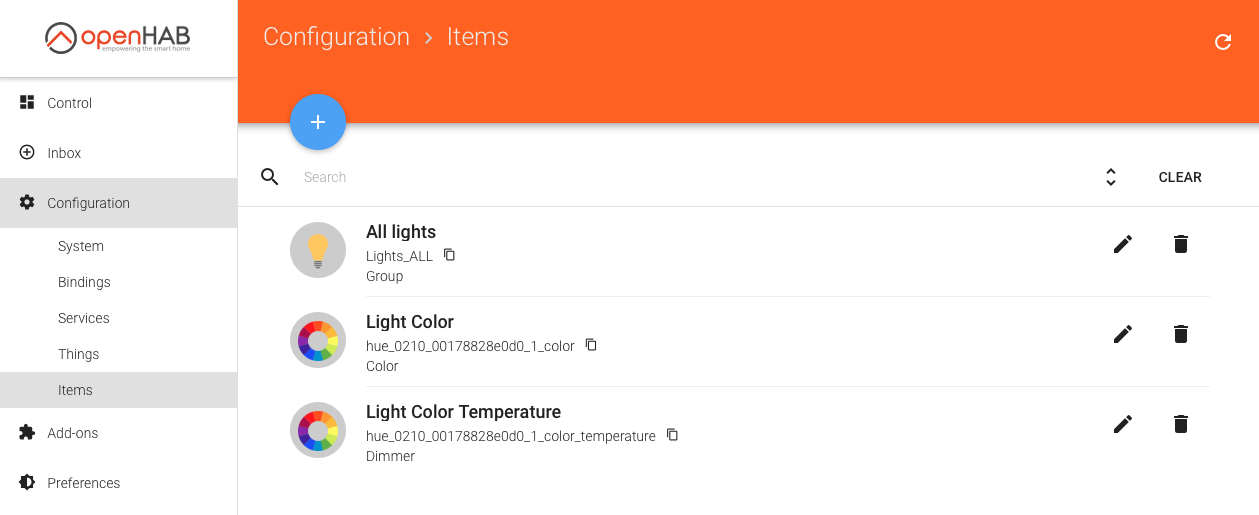
\includegraphics[width=1\textwidth]{images/Chapter_06/group-definition-paperui.png}
	\caption{Definition of group Items in PaperUI, OpenHAB 2}
	\label{fig:group-definition-paperui}
\end{figure}

Once we have these items grouped in PaperUI, it is recommendable to check if everything is working OK and ready to receive commands
from the assistant. A GET request to the following URL:\\
\begin{center}
	\textit{http://192.168.30.103:8080/rest/items?recursive=false}\\
\end{center}
Returns the following JSON, assuming that 192.168.30.103 is the IP of the machine.

\begin{lstlisting}[style=Consola]
[
  {
    "link": "http://192.168.30.103:8080/rest/items/hue_0210_00178828e0d0_1_color",
    "state": "OFF",
    "type": "Color",
    "name": "hue_0210_00178828e0d0_1_color",
    "label": "Light Color",
    "category": "colorwheel",
    "tags": [],
    "groupNames": [
      "Lights_ALL"
    ]
  },
  {
    "link": "http://192.168.30.103:8080/rest/items/hue_0210_00178828e0d0_1_color_temperature",
    "state": "OFF",
    "type": "Dimmer",
    "name": "hue_0210_00178828e0d0_1_color_temperature",
    "label": "Light Color Temperature",
    "category": "colorwheel",
    "tags": [],
    "groupNames": [
      "Lights_ALL"
    ]
  },
  {
    "members": [],
    "link": "http://192.168.30.103:8080/rest/items/Lights_ALL",
    "state": "OFF",
    "type": "Group",
    "name": "Lights_ALL",
    "label": "All lights",
    "category": "light",
    "tags": [],
    "groupNames": []
  }
]
\end{lstlisting}

As we can see, all the specified items are working and accessible from the REST API. As the script sends PUT requests to this API,
we can tell that it will reach the group and change all the states of its members.

Finally, the script that manages the assistant should be modified according to the number of groups the user has created, and their
names. We will explore this further in the following section.

\subsubsection{Final Result}
The final script triggers the assistant by pressing the button and by saying “OK Google”, has some customized commands for power
and OpenHAB management, and supports responses in a variety of languages. But there is still room to improve, as we will state in the
next section.

\subsection{Improving Command Processing}
The current structure of the custom assistant script can recognize portions (substrings) on the transcribed command. Although this
solution works, it requires the user to know exactly what to say to trigger his or her desired command, losing all the flexibility
that an assistant can have. Moreover, it is a very clumsy solution if we would like to add more custom commands, and they substitute
the actions that Google Assistant can perform given the same command. So, the challenge now is to complete the following points:
\begin{itemize}
	\item \textbf{Create a more flexible assistant}: make the assistant perform the same action from a broad range of different
	commands with the same meaning.
	\item \textbf{Make the assistant more extendible}: modularize and optimize the current script so it is easier to add more commands.
	Do not force the assistant to check all the possible commands after making the transcription.
	\item \textbf{Do not substitute any command that the Google Assistant could perform}: we want to keep the Google Assistant, but
	adding a layer for controlling OpenHAB. To avoid substituting the Google Assistant commands with our own custom commands,
	one possibility is to define another \textit{hotword}, so that we can use it to access our custom commands.
\end{itemize}

For this purpose, we can define a simple grammar that is going to help us to process the commands and will make possible to cover
all the previous points.

\begin{figure}
	\centering
	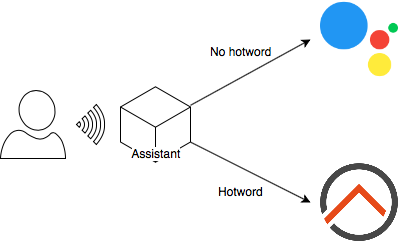
\includegraphics[width=0.65\textwidth]{images/Chapter_06/custom-assistant-simple.png}
	\caption{Basic diagram of the custom voice assistant}
	\label{fig:custom-assistant-simple}
\end{figure}

\subsubsection{Grammar Definition}
According to the Speech Recognition Grammar Specification v1.0 by the W3C, a token is typically an orthographic entity of the language 
being recognized. In the field of speech recognition, tokens can have a variety of forms (a single word, a number, a pair of words…),
but they all need to go through the same process, composed by: tokenization, white space normalization, token normalization and
pronunciation lookup.\cite{w3SpeechGrammar}

In our script, the Assistant Library takes care of this and returns us a clean, clutter-free string with the spoken phrase. But we
will consider tokens from another perspective for the next step: command processing.

First of all, we are going to define a \textit{hotword}, this is, a word or a couple of words that can identify the whole range of
available commands that we have defined to manage OpenHAB, so after the assistant identifies it, it can discard triggering Google
Assistant. It could be placed at the beginning of the sentence (prefixal), in the middle of it (infixal) or at the end (suffixal).
In this case, we are going to consider only the prefixal placement, so we let Google Assistant to process all the other sentences,
even if they have the hotword placed elsewhere.

The hotword that we are going to use is \textit{home}. It is easily recognizable by the assistant and cannot produce much confusion
in its pronunciation.

The hotword will be followed by a sentence whose form will be more or less free. At this point, trying to identify a substring of
more than two words is not very useful, so we can check for some keywords inside the sentence and discard the other options, step
by step. For that, we need to know how sentences are formed. In our case, the most common form will be as indicated in table
\ref{table:sentence-form-assistant}.

\begin{table}[]
	\centering
	\resizebox{\textwidth}{!}{%
		\begin{tabular}{|
				>{\columncolor[HTML]{C0C0C0}}c
				>{\columncolor[HTML]{C0C0C0}}c | ccc |}
			\hline
			\textbf{OK Google!} & \textbf{Hotword} & \begin{tabular}[c]{@{}c@{}}\textbf{Verb}\\ \textit{What to do}\end{tabular} & \begin{tabular}[c]{@{}c@{}}\textbf{Noun}\\ \textit{What to change}\end{tabular} & \begin{tabular}[c]{@{}c@{}}\textbf{Adjective}\\ \textit{To which state}\end{tabular} \\ \hline
		\end{tabular}%
	}
	\caption{Example sentence form for the assistant}
	\label{table:sentence-form-assistant}
\end{table}

So, the assistant has to process the part that goes right after the \textit{hotword}. In this case, we are going to check for actions,
like \textit{turn} or \textit{power}. If the action is contained anywhere in the sentence, it will check for derived words. For
example, it makes sense to check for \textit{on} or \textit{off} after these previous words. But before that, just to keep the
specified order, we will check the noun. In other words, the device to which the action is directed. As the script checks only if
the word is contained in the sentence, the order that it follows for checking words is not a big issue. But why does not it keep
track of the order?

\begin{enumerate}
	\item “Turn on all the lights”
	\item “Turn all the lights on”\\

	\item “Set the office light to red”
	\item “Turn red the office light”
\end{enumerate}

The sentences 1 and 2 and, on the other hand, the sentences 3 and 4, mean exactly the same. In an assistant that expects to receive
a relatively small amount of commands, this should be enough, though in more complex assistants checking the word order matters.

The sentence check will always end with the execution of a function. If it recognizes the correct words, it will trigger an OpenHAB
command or a system one, for example. If the sentence does not match what the assistant expects, it will say that the command has
not been recognized, in any case. To give it a more \textit{human} touch, it will exactly say \textit{Sorry, I cannot do that yet}.

We can see that this way we can extend a lot the functionality of the assistant, while keeping a well-organized code. Despite it
might have to do more checks than the previous version in some cases, in the long run with more commands, this will be
much more efficient, because it has the ability to discard many other options and go straight to the requested command.

Although we have tried to make a user-friendly script, it is clear that any house arrangement will need a specific configuration in
the script, depending on the devices and states that they can have.

\subsubsection{Improving the Range of Actions}
At this moment, the assistant is able to turn on and off all the lights and to manage the system (shutting down and rebooting).

Taking advantage of the improved command processing that we have specified above, we have implemented a few more actions. The following
example has been made over a system composed by a Philips HUE color light. It is really easy to implement more lights; the user just
needs to add their item IDs and a name for each light to the beginning of the file. The script will automatically recognize them,
and it will be able to send commands to them. Now, the actions that it can perform are:
\begin{itemize}
	\item For all the lights (through a \textit{Group} item):
	\begin{itemize}
		\item Turn on and off.
	\end{itemize}
	\item For each light:
	\begin{itemize}
		\item Turn on and off.
		\item Change the light color (red, yellow, blue, pink, green), maintaining its brightness.
		\item Change the light color temperature (cold, warm, natural).
		\item Increase and decrease its brightness.
	\end{itemize}
	\item For the system:
	\begin{itemize}
		\item Turn off.
		\item Reboot.
	\end{itemize}
\end{itemize}

The last three commands specific to a single light require a new function, which makes a GET request to the REST API of OpenHAB,
in order to get the current state of a light. The state of a Philips HUE light is composed by three numbers: its color (defined
between 0 and 360 degrees, like a color wheel), its saturation and its brightness (between 0 and 100). On each POST request, we need
to send these three values, so the script uses GET requests to send the same value that it had before in the parameters that we want
to maintain. This new function is really simple, and it uses the Python \textit{Requests} library.\cite{requestsDocumentation}

\begin{lstlisting}[style=PythonCode]
def openhab_get_state(item):
  url = 'http://localhost:8080/rest/items/' + item + '/state'
  r = requests.get(url)
  return r.text
\end{lstlisting}

\subsubsection{Final Result}
The full script is included in the appendix A.

\subsection{Adding Automation via IFTTT}
An often desirable function of a home automation system is the possibility to add and manage rules. Rules enable users to set actions
when a specific situation happens, so they do not have to interact directly with the system to perform these actions. This is called
automation, and an example of it can be lowering the shutters after 8 PM or turning on the house lights when a motion detector
perceives movement.

\subsubsection{Introduction to IFTTT}
There is a free platform that has become more popular over the last years called “If This Then Else”, or IFTTT. This web-based
service allows users to create chains of conditional statements, known as applets, and they can be really powerful. A conditional
statement could be one of the conditions mentioned above.\cite{iftttWebsite}

Apart from the website, IFTTT offers an application for iOS and Android, and integration with openHAB, which is the most interesting
part for us. Additionally, it is possible to connect other web services to IFTTT, such as social networks, and it is possible to use
them as well to trigger actions in OpenHAB.

The main disadvantage of IFTTT and other similar solutions is that the rule must be implemented to use it, and the user may not be
able to carry out the automation the way he wants. However, there are plenty of rules that can meet most requirements.

\subsubsection{OpenHAB and IFTTT}
As we can see, IFTTT perfectly complements OpenHAB, adding a functionality that, in spite of being present in other proprietary
home automation solutions, has many more possibilities.

IFTTT is available to all openHAB users through myopenHAB, which is an instance of the openHAB Cloud Service hosted by the openHAB
foundation. Thanks to this service, us and other apps can access and interact with our openHAB instance from the
Internet.\cite{openHABIftttDocs}

\subsubsection{Installation and Configuration}
By default, openHAB cannot connect to any openHAB Cloud instance, but there is a binding named \textit{openHAB Cloud Connector}
that we can install for this purpose. The binding is installed through the PaperUI. After this, two new files are created in the installation
folder of openHAB, in this case:

\begin{lstlisting}[style=Consola]
/var/lib/openhab2/uuid
/var/lib/openhab2/openhabcloud/secret
\end{lstlisting}

These files contain the UUID and secret key of the instance of openHAB. We need to create an account on myopenHAB, indicating an
email, password and these previous keys. Once the account is created, we can go back to our instance of the platform and configure
the binding (under \textit{Configuration $>$ Services $>$ IO $>$ openHAB Cloud}).

\begin{figure}
	\centering
	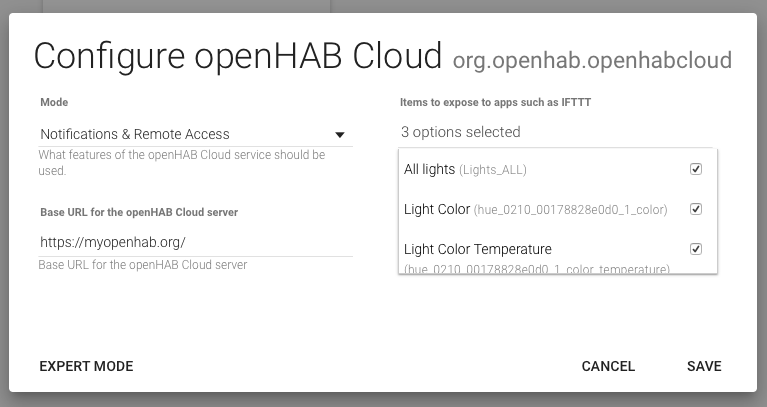
\includegraphics[width=1\textwidth]{images/Chapter_06/openhab-cloud-binding-conf.png}
	\caption{openHAB Cloud Binding configuration}
	\label{fig:openhab-cloud-binding-conf}
\end{figure}

The user must add some items to expose so IFTTT can manage them. Then, back to myopenHAB, we should be able to see the panel
of our instance. Thanks to this service, it is now accessible as well from any part of the world and to external services, like IFTTT.

After this, we have created an account on IFTTT, which is also a very quick process. Once the account is created, IFTTT shows a list
of the services that it is capable to handle. OpenHAB is between them, and we are taken back to myopenHAB to allow their connection.

Now, we are able to set IFTTT rules. We will set the first one on their web platform. The process begins with creating a new applet
of openHAB.

\begin{figure}
	\centering
	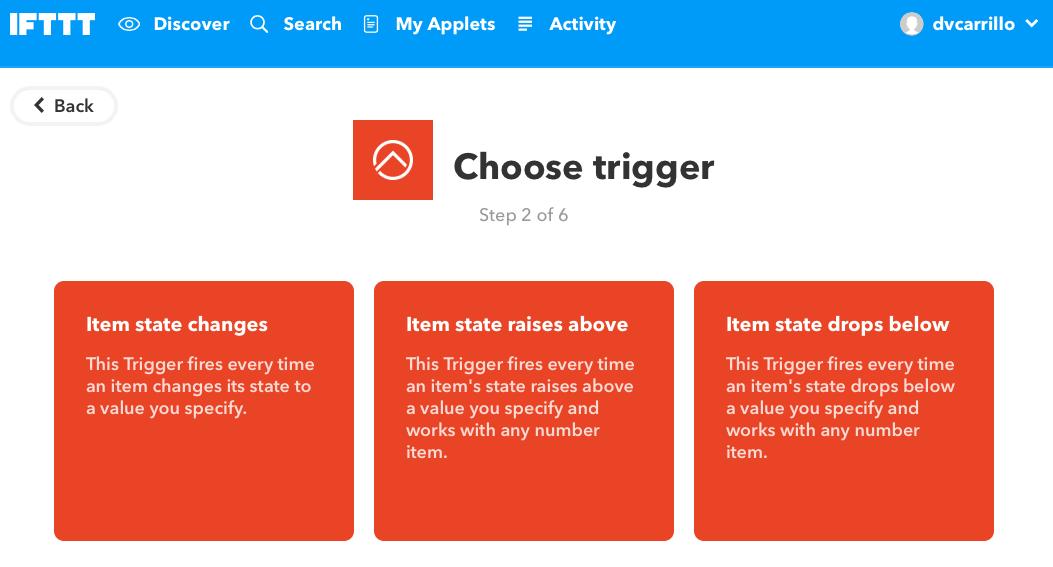
\includegraphics[width=1\textwidth]{images/Chapter_06/selection-iftt.png}
	\caption{Configuration of an openHAB IFTTT applet}
	\label{fig:selection-iftt}
\end{figure}

We can only select three different triggers, as shown in figure \ref{fig:selection-iftt}. In this example, we are going to make lights
turn blue if the humidity is over 70\%, so the if condition is going to be that \textit{item state raises above}. Then, we need to
specify the item (previously made accessible from openHAB), and give the minimum value, "70” in this case. After this, we are taken
back to the service selector, that offers us again a broad range of actions to accomplish if this condition happens. We choose again
openHAB, the item that is going to receive the command, and the command itself, which is simply: 260, 100, 100 (which turns the
light blue, at 100\% of brightness and saturation).

As this situation is not likely to happen in the moment we are writing these lines, we are going to set a new rule, which combines
openHAB and another service, like Twitter. Now the light is going to turn red every time we send a new tweet. We put Twitter as the
\textit{if condition} and openHAB in the \textit{then condition}. IFTTT is fully integrated with Twitter and includes very useful
shortcuts. However, with openHAB we need to write the full command, as if we were dealing with its REST API. This time, the command
that is sent to the light color item is pretty similar: 0, 100, 100 (zero indicates the red color, and the other parameters are the
same as in the previous command).

\begin{figure}
	\centering
	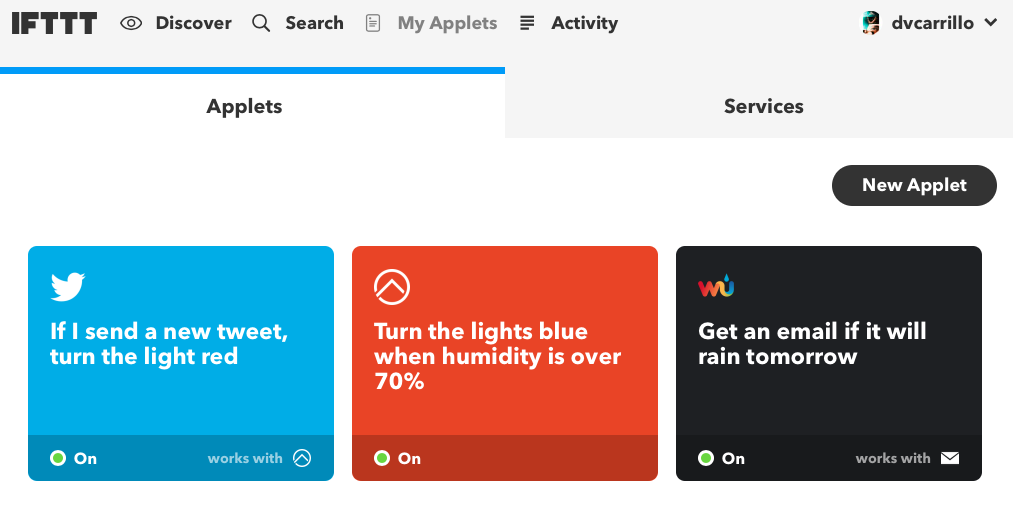
\includegraphics[width=1\textwidth]{images/Chapter_06/iftt-applet-panel.png}
	\caption{IFTTT applet panel}
	\label{fig:iftt-applet-panel}
\end{figure}

The applet works finely. We publish a tweet and, after some minutes, the light turns red. Although we have used this as an example,
it might not be really useful in a real environment, but the end user could use a similar rule as a notification system every time
he is mentioned on Twitter, or when he receives new emails. It is also possible to set very useful rules with the date and time as
the \textit{if condition}, like turning on the lights after 8 PM. Possibilities seem to be endless when combining openHAB and IFTTT.

\subsection{Adding Global Access to the System}
An openHAB instance can, by default, only be accessed from the same network as the device on which it is installed. This is also
the case in some other home automation systems and smart devices.

However, a home automation system that can be accessed from any place, regardless of the network the user is connected to, can
greatly extend its usability. For example, it would be possible to turn the oven on 30 minutes before arriving home and have the
food cooked at the moment the user arrives. Or checking the temperature inside home from the office.

In this section we will explore the different options we have to implement this feature, from doing it manually to making use of
the possibilities offered by openHAB.

\subsubsection{Making the Runtime Accessible From the Public Internet}
The first option is to make the local instance accessible from the public Internet. This is a process that can be done with any
software that is hosted in a computer connected to the Internet and that listens to any port and consists in making a route
between the device and its port, and the public Internet.\cite{nchPublicInternet}

In most homes and businesses, routers use a Network Address Translator, or a NAT, which is mainly what disallows to make devices
directly reachable from Internet. The NAT takes the public IP address for itself and assigns local IP addresses for the computers
and devices on the local network, so that they are all effectively sharing the same IP address. So, if we want to make a single
device reachable from outside, we need to tell the router how to address a specific request. This is called port forwarding and,
as the name indicates, it makes use of the ports. Ports are usually specific to each server-based application, and this is also the
case in openHAB, which uses the port 8080 by default.

Most of the routers nowadays provide a software where we can make any necessary change, which is accessible via HTTP in the local
address of the router. Here it is possible to set the ports that we want to forward.

\begin{figure}
	\centering
	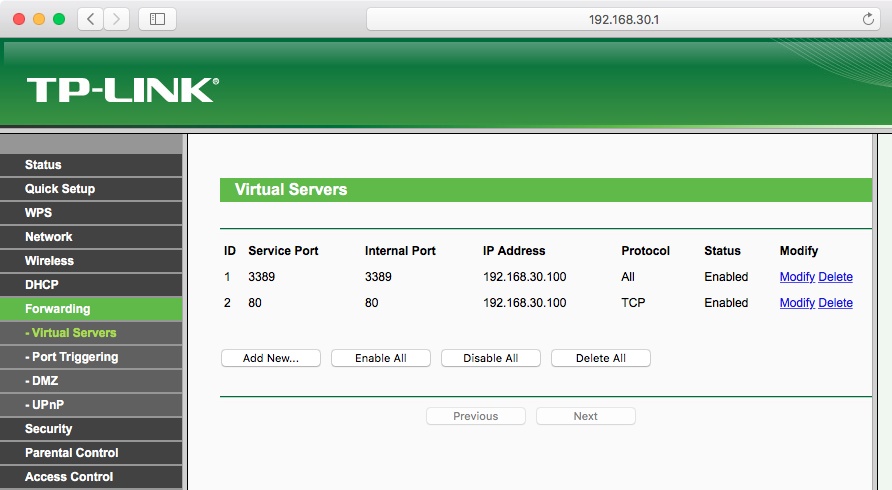
\includegraphics[width=1\textwidth]{images/Chapter_06/port-forwarding.png}
	\caption{Port Forwarding section of the router used in this project}
	\label{fig:port-forwarding}
\end{figure}

For setting a port forwarding rule we usually need to specify some properties, as the protocol to use, the start and end ports or
the host IP. After that, the router should be able to address any request with the specified properties to the device.

Although this is an easy and fast process, we will not go into detail too much, as this is a very unsafe solution. OpenHAB does
not provide any authentication method nor any restricted access at this moment, so opening a port must be avoided, because anyone
could access our system and view all data as if they were us.

\subsubsection{Running openHAB Behind a Reverse Proxy}
This solution will make our openHAB instance accessible from the Internet without depending on any third-party servers. However,
we need our own domain first. This solution is the best one if the user has already purchased a domain. If not, this would require
spending between EUR 10 and EUR 20 every year\cite{startBloggingDomainCost}, so it might be more appropriate to use myopenHAB
Cloud Service, which is free to use.

Running openHAB behind a reverse proxy allows to access the openHAB runtime via port 80 (HTTP) and 443 (HTTPS). It also provides a
simple way of protecting the server with authentication and secure certificates.

The first step is to set up a HTTP server, like NGINX or Apache, which support reverse proxying. NGINX is based on configuration
files, and we need to create one to allow it to proxy openHAB. The following code is the configuration to apply, as long as the
openHAB instance is located in the same machine as the reverse proxy, as in our case:

\begin{lstlisting}[style=Consola]
server {
  listen                                  80;
  server_name                             openhabpi.me;

  location / {
    proxy_pass                            http://localhost:8080/;
    proxy_set_header Host                 $http_host;
    proxy_set_header X-Real-IP            $remote_addr;
    proxy_set_header X-Forwarded-For      $proxy_add_x_forwarded_for;
    proxy_set_header X-Forwarded-Proto    $scheme;
  }
}
\end{lstlisting}

Then, we save the file in sites-available and \textit{activate}it by linking it in the sites-enabled folder. After it, we only need
to restart NGINX and it should be ready.

The system can be secured thanks to the authentication system that NGINX provides, which needs to be configured with an
authentication user file and with the utility htpasswd, included in the \textit{apache2-utils} package. The following command
creates a file that we can use with NGINX. We use \textit{dvcarrillo} as the username:

\begin{lstlisting}[style=Consola]
sudo htpasswd -c /etc/nginx/.htpasswd dvcarrillo
\end{lstlisting}

Once it has been created, we have to move it to the NGINX directory (in our case, \textit{/etc/nginx/sites-enabled/openhab}), and
include these lines in the configuration file, underneath the \textit{proxy\_*} settings:

\begin{lstlisting}[style=Consola]
auth_basic                     "Username and Password Required";
auth_basic_user_file           /etc/nginx/.htpasswd;
\end{lstlisting}

NGINX should be restarted to apply these changes now.

Another way to secure the system without needing to enter a username and password is to restrict the access to only some specific
IPs, blocking the access to everyone else. This can be done thanks to the NGINX directives \textit{satisfy} and \textit{deny}.
For example, by adding these lines inside the location block:

\begin{lstlisting}[style=Consola]
satisfy  any;
allow    192.168.0.1/24;
allow    127.0.0.1;
deny     all;
\end{lstlisting}

NGINX will allow anyone within the range from 192.168.0.1 to 192.168.0.24 and the \textit{localhost} to connect without a password.

To pick this method or the previous one is totally up to the user’s needs and his own idea of the system. The password authentication
is suitable if he wants to connect to his openHAB instance from several networks and he does not know their IP beforehand. But if
he knows exactly the networks and devices that he is going to use, the second option provides extra security.

Another option is to combine both, which would require to set up a password and then configure the IP allowance. This way, the
allowed IP addresses would directly access openHAB and the rest of them would be asked to log in using the specified username and
password.

The reverse proxy choice also provides, as mentioned, the possibility to enable HTTPS, so communications between the client and
the server are encrypted. This is an important step that will protect against eavesdropping and possible forgery, and it is highly
recommended to anyone who chooses this method.

The process to enable HTTPS in the reverse proxy begins with using OpenSSL to generate a self-signed certificate. Although if we
have a valid domain and can change the DNS to point towards your IP, openHAB recommends using Let’s Script.\cite{letsEncryptWebsite}

OpenSSL can generate a certificate which will be valid for a year with the following command:

\begin{lstlisting}[style=Consola]
sudo openssl req -x509 -nodes -days 365 -newkey rsa:2048 -keyout /etc/ssl/openhab.key -out /etc/ssl/openhab.cr
\end{lstlisting}

Then, we need to tell NGINX that there are SSL certificates and their location. This is done by adding the following to the
configuration file, underneath the \textit{server\_name} variable, assuming we placed the certificate in the directory \textit{/etc/ssl/}:

\begin{lstlisting}[style=Consola]
ssl_certificate                 /etc/ssl/openhab.crt;
ssl_certificate_key             /etc/ssl/openhab.key;
\end{lstlisting}

Then, we must tell the server to listen on the HTTPS port by changing the listen parameter:

\begin{lstlisting}[style=Consola]
listen                          443 ssl;
\end{lstlisting}

After restarting NGINX, we will be using a valid HTTPS certificate. Finally, we must redirect the HTTP traffic to HTTPS. To get this
done, we only need to tell the server to direct all incoming connections on the port 80 (http) to the https version of the domain.

\paragraph{Final Result}
To summarize, the final NGINX configuration file will look like the following:

\begin{lstlisting}[style=Consola]
server {
  listen                         80;
  server_name                    openhabpi.me;
  return 301                     https://$server_name$request_uri;
}
server {
  listen                         443 ssl;
  server_name                    openhabpi.me;

  ssl_certificate                /etc/ssl/openhab.crt
  ssl_certificate_key            /etc/ssl/openhab.key

  location / {
    proxy_pass                             http://localhost:8080/;
    proxy_set_header Host                  $http_host;
    proxy_set_header X-Real-IP             $remote_addr;
    proxy_set_header X-Forwarded-For       $proxy_add_x_forwarded_for;
    proxy_set_header X-Forwarded-Proto     $scheme;
    satisfy                                any;
    allow                                  192.168.0.1/24;
    allow                                  127.0.0.1;
    deny                                   all;
    auth_basic                             "Username and Password Required";
    auth_basic_user_file                   /etc/nginx/.htpasswd;
  }
}
\end{lstlisting}

This is the safest method we propose, and we believe that under normal circumstances, this security will be more than enough.
Although it can even be improved further, indicating specific cyphers and SSL settings. OpenHAB proposes the following snippet for
this purpose:

\begin{lstlisting}[style=Consola]
ssl_protocols                   TLSv1 TLSv1.1 TLSv1.2;
ssl_prefer_server_ciphers       on;
ssl_dhparam                     /etc/nginx/ssl/dhparam.pem;
ssl_ciphers                     ECDHE-ECDSA-AES256-GCM-SHA384:ECDHE-RSA-AES256-GCM-SHA384:ECDHE-ECDSA-AES256-SHA384:ECDHE-RSA-AES256-SHA384:ECDHE-ECDSA-AES128-GCM-SHA256:ECDHE-RSA-AES128-GCM-SHA256:ECDHE-ECDSA-AES128-SHA256:ECDHE-RSA-AES128-SHA256:ECDHE-RSA-AES256-SHA:HIGH:!aNULL:!eNULL:!LOW:!3DES:!MD5:!EXP:!CBC:!EDH:!kEDH:!PSK:!SRP:!kECDH;
ssl_session_timeout             1d;
ssl_session_cache               shared:SSL:10m;
keepalive_timeout               70;
\end{lstlisting}

\subsubsection{Using myopenHAB Cloud Service}
MyopenHAB is an instance of the openHAB Cloud service, which is hosted by the openHAB Foundation e.V.

This service is fully free and it is meant to allow users to quickly check out its features without having to set up and host a
personal instance.

Unlike the previous solution, this requires almost zero installation or configuration from the user, the set up process is easy
and fast. As mentioned in the previous IFTTT section, the openHAB Cloud Connector binding would allow our system to be reachable
from anywhere in the world, thanks to myopenHAB.

Then, the first step is to install the Cloud Connector bundle on the local openHAB runtime. This bundle establishes the connection
to myopenHAB.org and authenticates against it. After this, we can log in to myopenHAB website (\textit{https://myopenhab.org}).
This will give us remote web access to the web UIs of our openHAB instance and will also let us check for the state of the items,
notifications and events.

On the downside, the reliability of this service depends on third parties. They explicitly specify in their website\cite{myopenHAB}
that we must be aware that they cannot offer any SLAs regarding availability. However, they promise to keep it up and running to
the best of their capabilities.

\paragraph{Integration With the Mobile Application} The advantages of using myopenHAB are also related to the openHAB mobile application.
By default, we are able to access the system if we are connected to the local network where the openHAB server is located. However,
if we use myopenHAB and enter \textit{https://myopenhab.org} as a remote URL and the user and password in the credentials, we will
be able to manage the openHAB runtime from anywhere in the world, and from the mobile phone. This is a very positive point to
consider when choosing one of these options.

\subsubsection{Conclusion}
In this case, we will choose myopenHAB Cloud Service. After testing it, we have found it reliable enough for a domestic use, although
in other cases where we need to assure its functionality for the longest time, it is more recommendable to run openHAB behind a
reverse proxy. MyopenHAB is also free and easy to use, and its integration with the mobile application works perfectly.

However, we would never recommend using the first proposed solution (making the instance accessible from the public Internet), as
it presents major security problems.
